\documentclass{beamer}\usepackage[]{graphicx}\usepackage[]{color}
%% maxwidth is the original width if it is less than linewidth
%% otherwise use linewidth (to make sure the graphics do not exceed the margin)
\makeatletter
\def\maxwidth{ %
  \ifdim\Gin@nat@width>\linewidth
    \linewidth
  \else
    \Gin@nat@width
  \fi
}
\makeatother

\definecolor{fgcolor}{rgb}{0.345, 0.345, 0.345}
\newcommand{\hlnum}[1]{\textcolor[rgb]{0.686,0.059,0.569}{#1}}%
\newcommand{\hlstr}[1]{\textcolor[rgb]{0.192,0.494,0.8}{#1}}%
\newcommand{\hlcom}[1]{\textcolor[rgb]{0.678,0.584,0.686}{\textit{#1}}}%
\newcommand{\hlopt}[1]{\textcolor[rgb]{0,0,0}{#1}}%
\newcommand{\hlstd}[1]{\textcolor[rgb]{0.345,0.345,0.345}{#1}}%
\newcommand{\hlkwa}[1]{\textcolor[rgb]{0.161,0.373,0.58}{\textbf{#1}}}%
\newcommand{\hlkwb}[1]{\textcolor[rgb]{0.69,0.353,0.396}{#1}}%
\newcommand{\hlkwc}[1]{\textcolor[rgb]{0.333,0.667,0.333}{#1}}%
\newcommand{\hlkwd}[1]{\textcolor[rgb]{0.737,0.353,0.396}{\textbf{#1}}}%
\let\hlipl\hlkwb

\usepackage{framed}
\makeatletter
\newenvironment{kframe}{%
 \def\at@end@of@kframe{}%
 \ifinner\ifhmode%
  \def\at@end@of@kframe{\end{minipage}}%
  \begin{minipage}{\columnwidth}%
 \fi\fi%
 \def\FrameCommand##1{\hskip\@totalleftmargin \hskip-\fboxsep
 \colorbox{shadecolor}{##1}\hskip-\fboxsep
     % There is no \\@totalrightmargin, so:
     \hskip-\linewidth \hskip-\@totalleftmargin \hskip\columnwidth}%
 \MakeFramed {\advance\hsize-\width
   \@totalleftmargin\z@ \linewidth\hsize
   \@setminipage}}%
 {\par\unskip\endMakeFramed%
 \at@end@of@kframe}
\makeatother

\definecolor{shadecolor}{rgb}{.97, .97, .97}
\definecolor{messagecolor}{rgb}{0, 0, 0}
\definecolor{warningcolor}{rgb}{1, 0, 1}
\definecolor{errorcolor}{rgb}{1, 0, 0}
\newenvironment{knitrout}{}{} % an empty environment to be redefined in TeX

\usepackage{alltt}

\def\currentCourse{An introduction to graph analysis and modeling}
\def\currentInstitute{MSc in Statistics for Smart Data -- ENSAI}
\def\currentLogo{../common_figs/logo_ensai}
\def\currentDate{Automn semester, 2018}
\def\currentChapter{Descriptive Analysis of Network Data}


% THEME BEAMER
\usepackage{../beamer_theme}

\graphicspath{{figures/},{../common_figs/}}

\usepackage{multirow}
\usepackage{tikz}
\usepackage[vlined]{algorithm2e}

\pgfdeclareimage[width=.5cm]{computer}{computer.png}

% \usetikzlibrary{calc,shapes,backgrounds,arrows,automata,shadows,positioning}
% \tikzstyle{every state}=[fill=red,draw=none,scale=0.7,font=\small,text=white]
% \tikzstyle{every edge}=[-,shorten >=1pt,auto,thin,draw]
% \tikzstyle{alertstate}=[fill=bleu]
% \definecolor{genecolor}{RGB}{94,135,173}

\title{\currentCourse}

\subtitle{\huge\currentChapter\normalsize}

\institute{\currentInstitute}

\date{\currentDate}



\AtBeginSection{
  \begin{frame}<beamer>
    \frametitle{Outline}
    \framesubtitle{\insertpart}
    \tableofcontents[currentsection,currentsubsection, subsectionstyle=show/shaded/hide]  
  \end{frame}
}

\AtBeginSubsection{
  \begin{frame}<beamer>
    \frametitle{Outline}
    \framesubtitle{\insertpart}
    \tableofcontents[currentsection,currentsubsection, subsectionstyle=show/shaded/hide]  
  \end{frame}
}

\AtBeginSubsubsection{
  \begin{frame}<beamer>
    \frametitle{Outline}
    \framesubtitle{\insertpart}
    \tableofcontents[currentsection,currentsubsection, subsectionstyle=show/shaded/hide]  
  \end{frame}
}

\newcommand{\dotitlepage}{%
  \begin{frame}
    \titlepage
    \vfill
    \begin{center}
        \scriptsize\url{https://github.com/jchiquet/CourseStatNetwork}
    \end{center}
    \vfill
    \includegraphics[width=2cm]{\currentLogo}\hfill
    
\includegraphics[width=2.5cm]{logo_inra}
  \end{frame}
  %
}

\newcommand{\dotoc}{%
  \begin{frame}
    \frametitle{Outline}
    \tableofcontents[currentsection,
    sectionstyle=show/show,
    subsectionstyle=hide]
  \end{frame}
  %
}



\usetikzlibrary{calc,shapes,backgrounds,arrows,automata,shadows,positioning}
\IfFileExists{upquote.sty}{\usepackage{upquote}}{}
\begin{document}

\dotitlepage

\begin{frame}
  \frametitle{Outline}
  \tableofcontents
\end{frame}

%% ==========================================================================
\section{Basic notions on graphs and networks}
%% ==========================================================================

\begin{frame} 
  \frametitle{References}

    \begin{thebibliography}{99}
      \setbeamertemplate{bibliography item}[book]

    \bibitem[EK2]{EK2} Statistical Analysis of Network Data: Methods and Models, 
    \newblock \textcolor{black}{Eric Kolazcyk} 
    \newblock \alert{Chapiter 2, Section 1}

      \setbeamertemplate{bibliography item}[article]

    \bibitem[CM1]{CM1} Analyse statistique de graphes, 
    \newblock \textcolor{black}{Catherine Matias}
    \newblock \alert{Chapitre 1}    

    \end{thebibliography}

\end{frame}

\subsection{Definitions}

\begin{frame}
  \frametitle{Graphs, Networks: some definitions}

  \begin{definition}[Network versus Graph]
    \vspace{-.25cm}
    \begin{itemize}
      \item  A \alert{Network} is a collection of interacting entities
      \item  A \alert{Graph} is the mathematical representation of a network
    \end{itemize}
  \end{definition}

  \vfill

  \begin{definition}[Graph]
    A graph $\clG=(\clV,\clE)$ is a mathematical structure consisting of
    \begin{itemize}
      \item a set $\clV=\set{1,\dots,n}$ of \alert{vertices} or \alert{nodes} 
      \item a set $\clE=\set{e_1,\dots,e_p:e_k=(i_k,j_k)\in (\clV\times\clV)}$ of \alert{edges} or \alert{links} 
      \item The number of vertices $N_v=|\clV|$ is called the \alert{order}
      \item The number of edges $N_e=|\clE|$ is called the \alert{size}
    \end{itemize}
  \end{definition}

\end{frame}

\begin{frame}
  \frametitle{Graphs, Networks: some vocabulary}

  \begin{block}{Not comprehensive}
    \begin{itemize}
      \item subgraph $\clH = (\clV_\clH, \clE_\clH)$, 
      \item  induced subgraph
      \item (un)directed graph, 
      \item  weighted graph, 
      \item  bipartite graph, 
      \item  tree, 
      \item  DAG, etc.
    \end{itemize}
  \end{block}

\end{frame}

\begin{frame}[fragile]
\frametitle{Examples}
\framesubtitle{Undirected, directed (digraph), complete, bipartite}

\begin{knitrout}\scriptsize
\definecolor{shadecolor}{rgb}{0.969, 0.969, 0.969}\color{fgcolor}
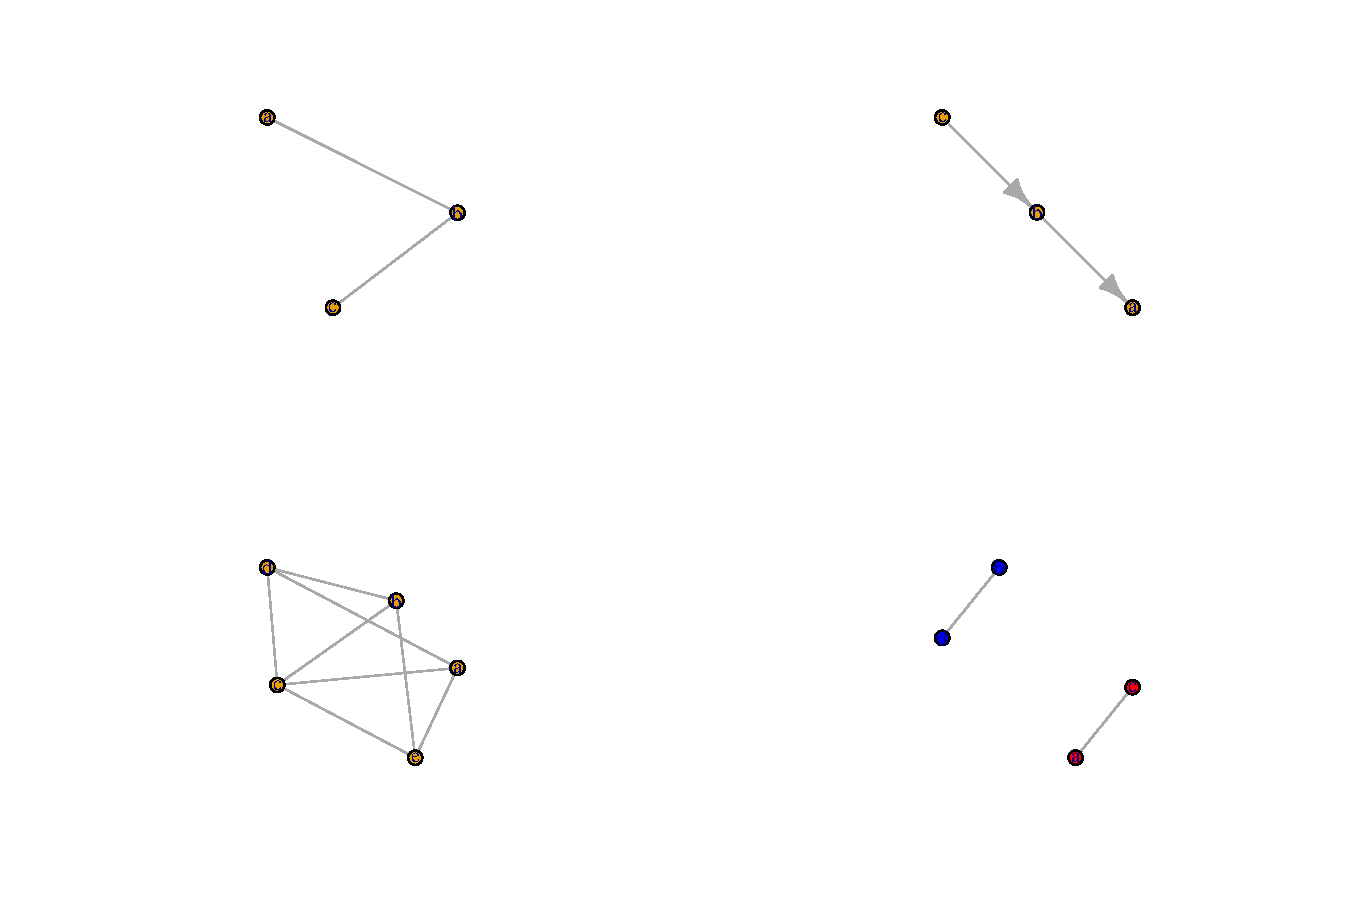
\includegraphics[width=.8\textwidth]{figures/basic_graphs-1} 

\end{knitrout}

\end{frame}

\begin{frame}[allowframebreaks]
  \frametitle{Paths, Cycles, Connected Components}

  \begin{definition}[Path]
    In a undirected graph $\clG = (\clV,\clE)$ a path  between $i,j\in \clV^2$ is a series of edges $e_1,\dots,e_k$ such that
    \begin{itemize}
      \item  $\forall 1 \leq \ell < k$, all edges $(e_\ell, e_{\ell+1})$ share a vertex in $\clV$
      \item  $e_1$ starts from $i$, $e_k$ ends to $j$.
    \end{itemize}
  \end{definition}

  \begin{block}{Vocabulary}
    \vspace{-.25cm}
    \begin{itemize}
    \item  A \alert{cycle} is a path from $i$ to itself.
    \item  A \alert{connected component} is a subset $\clV'\subset\clV$ such that there exists an path between any $i,j\in\clV'$.
    \item A graph is \alert{connected} when there is a path between every pairs of vertices.
    \end{itemize}
  \end{block}

  \begin{proposition}[Decomposition]
    Any graph can be decomposed in a unique set of maximal connected components. The number of connected component is a least $n - |\clE|$
  \end{proposition}

\end{frame}

\begin{frame}
  \frametitle{Neighborhood, Degree}

  \begin{definition}[Neighborhood]
    The neighbors of a vertex are the nodes directly connected to this vertex:
    \[
      \clN(i) = \set{j\in\clV : (i,j) \in \clE}.
    \]
  \end{definition}
  
  \begin{definition}[Degree]
    The degree $d_i$ of a node $i$ is given by its number of neighbors, i.e. $|\clN(i)|$.
  \end{definition}

  \begin{block}{Remark}
    In digraphs, vertex degree is replaced by \alert{in-degree} and \alert{out-degree}.
  \end{block}

  \begin{proposition}
    In a graph $\clG = (\clV,\clE)$ the sum of the degree is given by $2|\clE|$. Hence \alert{this is always an even quantity}.
  \end{proposition}
  
  
\end{frame}

\subsection{Representations}

\begin{frame}
  \frametitle{Adjacency matrix and list of edges}

  \begin{definition}[Adjacency matrix]
    The connectivity of  $\clG = (\clV,\clE)$ is captured by the $|\clV|\times |\clV|$ matrix $\bA$:
    \[
      (\bA)_{ij} = \begin{cases}
      1  & \text{ if } i \sim j,\\
      0  & \text{otherwise}.
      \end{cases}
    \]
  \end{definition}

  \begin{proposition}
    The degree of $\clG$ are then simply obtained as the row-wise and/or column-wise sums of $\bA$.
  \end{proposition}

  \begin{block}{Remark}
    If the list of vertices is known, the only information which needs to be stored is the list of edges. In terms of storage, this is equivalent to a sparse matrix representation.
  \end{block}
  
\end{frame}

\begin{frame}
  \frametitle{Incidence matrix}

  \begin{definition}[Incidence matrix]
    The connectivity of $\clG = (\clV,\clE)$ is captured by the $|\clV|\times |\clE|$ matrix $\bB$:
    \[
      (\bB)_{ij} = \begin{cases}
      1  & \text{ if $i$ is incident to edge $j$},\\
      0  & \text{otherwise}.
      \end{cases}
    \]
  \end{definition}

  \begin{proposition}[Relationship]
    Let $\tilde\bB$ be a modified \alert{signed} version of $\bB$ where $\tilde{\! B}_{ij}= 1/-1$ if $i$ is incident to $j$ as tail/head. Then
    \[
      \tilde \bB \tilde \bB^\intercal = \bD - \bA,
    \]
    where $\bD = \diag(\set{d_i, i\in\clV})$ is the diagonal matrix of degrees. 
  \end{proposition}

  $\rightsquigarrow \tilde \bB \tilde \bB^\intercal $ is called the Laplacian matrix and will be studied latter.

\end{frame}


\begin{frame}
  \frametitle{Layout and Vizualization}
  
  \begin{itemize}
    \item Vizualization of large networks is a field of research in its own
    \item Be carefull with graphical interpretation of (large) networks
  \end{itemize}

\begin{knitrout}\scriptsize
\definecolor{shadecolor}{rgb}{0.969, 0.969, 0.969}\color{fgcolor}\begin{kframe}
\begin{alltt}
\hlkwd{library}\hlstd{(igraph)}

\hlkwd{library}\hlstd{(sand)}

\hlstd{GLattice} \hlkwb{<-} \hlkwd{graph.lattice}\hlstd{(}\hlkwd{c}\hlstd{(}\hlnum{5}\hlstd{,}\hlnum{5}\hlstd{,}\hlnum{5}\hlstd{))}

\hlstd{GBlog}    \hlkwb{<-} \hlstd{aidsblog}
\end{alltt}
\end{kframe}
\end{knitrout}
  
\end{frame}

\begin{frame}
  \frametitle{Layout and Vizualization}
  \framesubtitle{Example with circle plot}
  


\begin{knitrout}\scriptsize
\definecolor{shadecolor}{rgb}{0.969, 0.969, 0.969}\color{fgcolor}\begin{kframe}
\begin{alltt}
\hlkwd{par}\hlstd{(}\hlkwc{mfrow}\hlstd{=}\hlkwd{c}\hlstd{(}\hlnum{1}\hlstd{,}\hlnum{2}\hlstd{))}

\hlkwd{plot}\hlstd{(GLattice,} \hlkwc{layout}\hlstd{=layout.circle);} \hlkwd{title}\hlstd{(}\hlstr{"5x5x5 lattice"}\hlstd{)}

\hlkwd{plot}\hlstd{(GBlog   ,} \hlkwc{layout}\hlstd{=layout.circle);} \hlkwd{title}\hlstd{(}\hlstr{"blog network"}\hlstd{)}
\end{alltt}
\end{kframe}
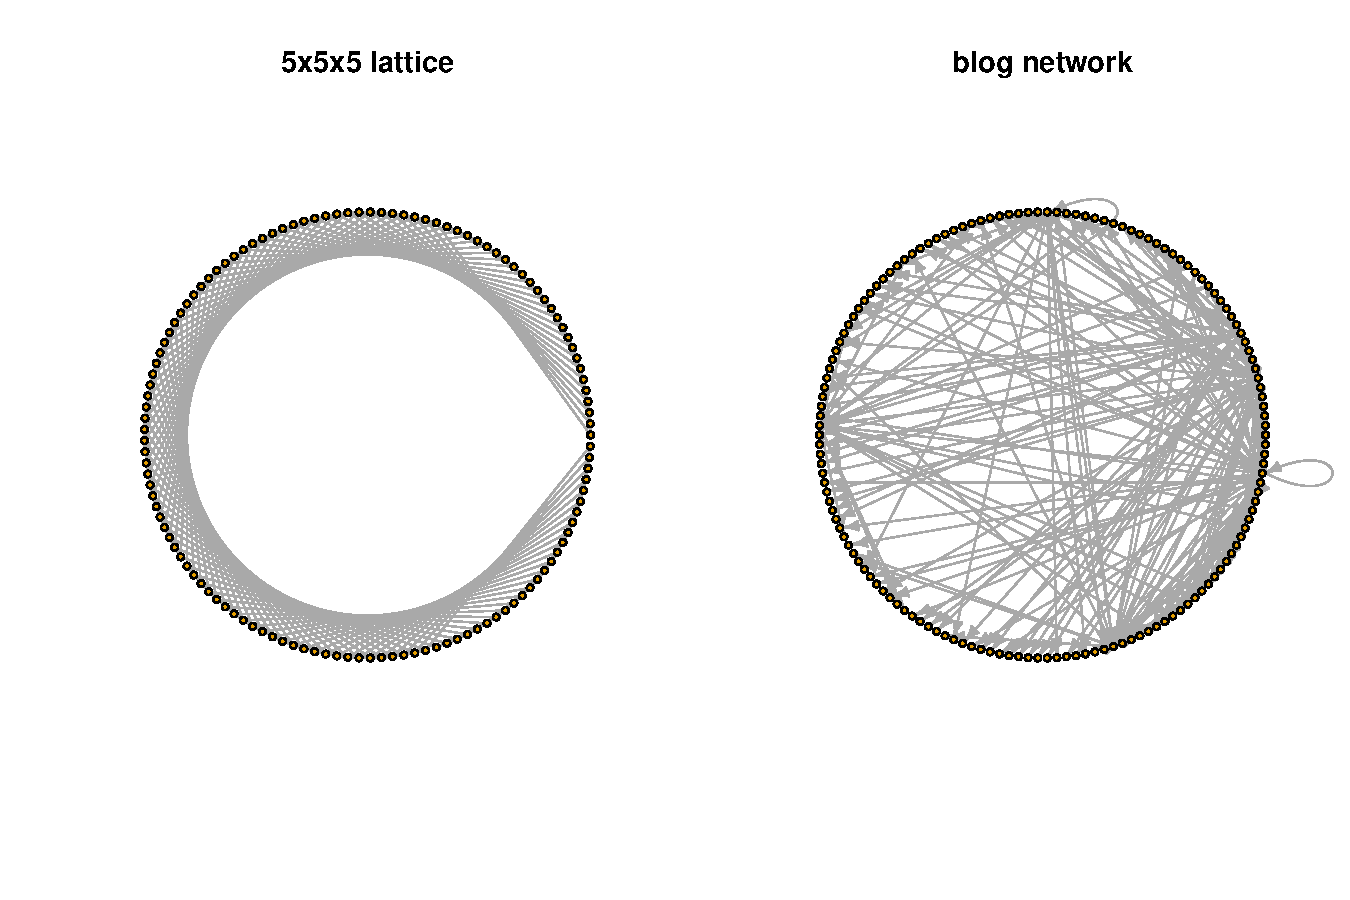
\includegraphics[width=.8\textwidth]{figures/vizu_3-1} 

\end{knitrout}
  
\end{frame}

\begin{frame}
  \frametitle{Layout and Vizualization}
  \framesubtitle{Example with Fruchterman and Reingold}

\begin{knitrout}\scriptsize
\definecolor{shadecolor}{rgb}{0.969, 0.969, 0.969}\color{fgcolor}\begin{kframe}
\begin{alltt}
\hlkwd{par}\hlstd{(}\hlkwc{mfrow}\hlstd{=}\hlkwd{c}\hlstd{(}\hlnum{1}\hlstd{,}\hlnum{2}\hlstd{))}

\hlkwd{plot}\hlstd{(GLattice,} \hlkwc{layout}\hlstd{=layout.fruchterman.reingold);} \hlkwd{title}\hlstd{(}\hlstr{"5x5x5 lattice"}\hlstd{)}

\hlkwd{plot}\hlstd{(GBlog   ,} \hlkwc{layout}\hlstd{=layout.fruchterman.reingold);} \hlkwd{title}\hlstd{(}\hlstr{"blog network"}\hlstd{)}
\end{alltt}
\end{kframe}
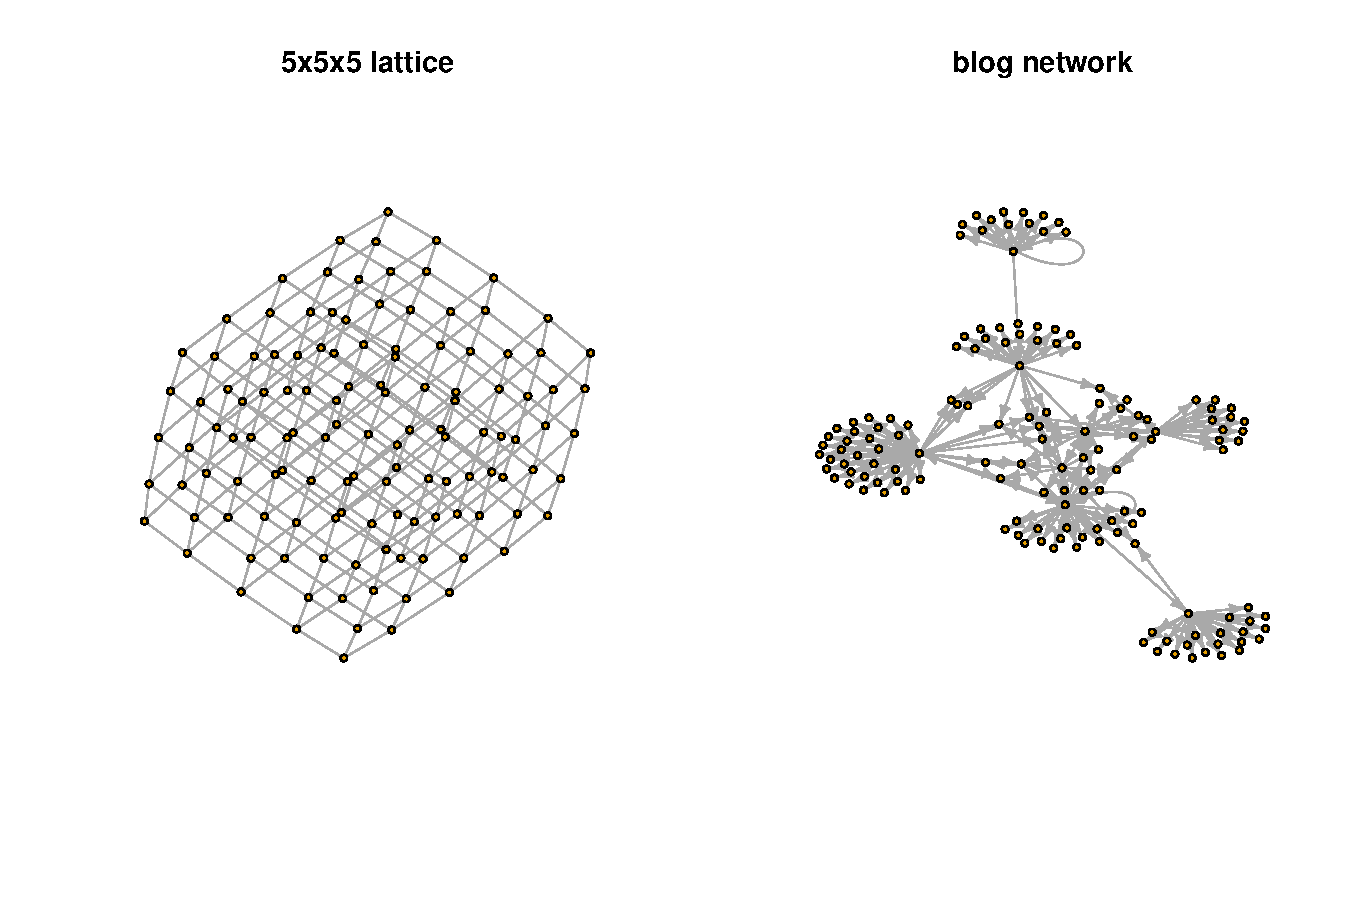
\includegraphics[width=.8\textwidth]{figures/vizu_4-1} 

\end{knitrout}
  
\end{frame}

\begin{frame}[fragile, allowframebreaks]
  \frametitle{Layout and Vizualization: \textbf{ggraph} way}
 
\begin{knitrout}\scriptsize
\definecolor{shadecolor}{rgb}{0.969, 0.969, 0.969}\color{fgcolor}\begin{kframe}
\begin{alltt}
\hlkwd{library}\hlstd{(ggraph)}
\hlkwd{library}\hlstd{(gridExtra)}
\hlstd{g1} \hlkwb{<-} \hlkwd{ggraph}\hlstd{(GBlog,} \hlkwc{layout} \hlstd{=} \hlstr{"fr"}\hlstd{)} \hlopt{+}
  \hlkwd{geom_edge_link}\hlstd{(}\hlkwc{color} \hlstd{=} \hlstr{"lightgray"}\hlstd{)} \hlopt{+} \hlkwd{geom_node_point}\hlstd{()} \hlopt{+} \hlkwd{theme_void}\hlstd{()}

\hlstd{g2} \hlkwb{<-} \hlkwd{ggraph}\hlstd{(GBlog   ,} \hlkwc{layout} \hlstd{=} \hlstr{"kk"}\hlstd{)} \hlopt{+}
  \hlkwd{geom_edge_link}\hlstd{(}\hlkwc{color} \hlstd{=} \hlstr{"lightgray"}\hlstd{)} \hlopt{+} \hlkwd{geom_node_point}\hlstd{()} \hlopt{+} \hlkwd{theme_void}\hlstd{()}

\hlstd{g3} \hlkwb{<-} \hlkwd{ggraph}\hlstd{(GBlog,} \hlkwc{layout} \hlstd{=} \hlstr{"linear"}\hlstd{)} \hlopt{+}
  \hlkwd{geom_edge_arc}\hlstd{(}\hlkwd{aes}\hlstd{(}\hlkwc{alpha}\hlstd{=..index..),} \hlkwc{show.legend} \hlstd{=} \hlnum{FALSE}\hlstd{)} \hlopt{+}
  \hlkwd{geom_node_point}\hlstd{()} \hlopt{+} \hlkwd{theme_void}\hlstd{()}

\hlstd{g4} \hlkwb{<-} \hlkwd{ggraph}\hlstd{(GBlog   ,} \hlkwc{layout} \hlstd{=} \hlstr{"linear"}\hlstd{,} \hlkwc{circular} \hlstd{=} \hlnum{TRUE}\hlstd{)} \hlopt{+}
  \hlkwd{geom_edge_link}\hlstd{(}\hlkwd{aes}\hlstd{(}\hlkwc{alpha}\hlstd{=..index..),} \hlkwc{show.legend} \hlstd{=} \hlnum{FALSE}\hlstd{)} \hlopt{+}
  \hlkwd{geom_node_point}\hlstd{()} \hlopt{+} \hlkwd{theme_void}\hlstd{()}

\hlkwd{grid.arrange}\hlstd{(g1, g2, g3, g4,} \hlkwc{nrow} \hlstd{=} \hlnum{2}\hlstd{,} \hlkwc{ncol} \hlstd{=} \hlnum{2}\hlstd{)}
\end{alltt}
\end{kframe}
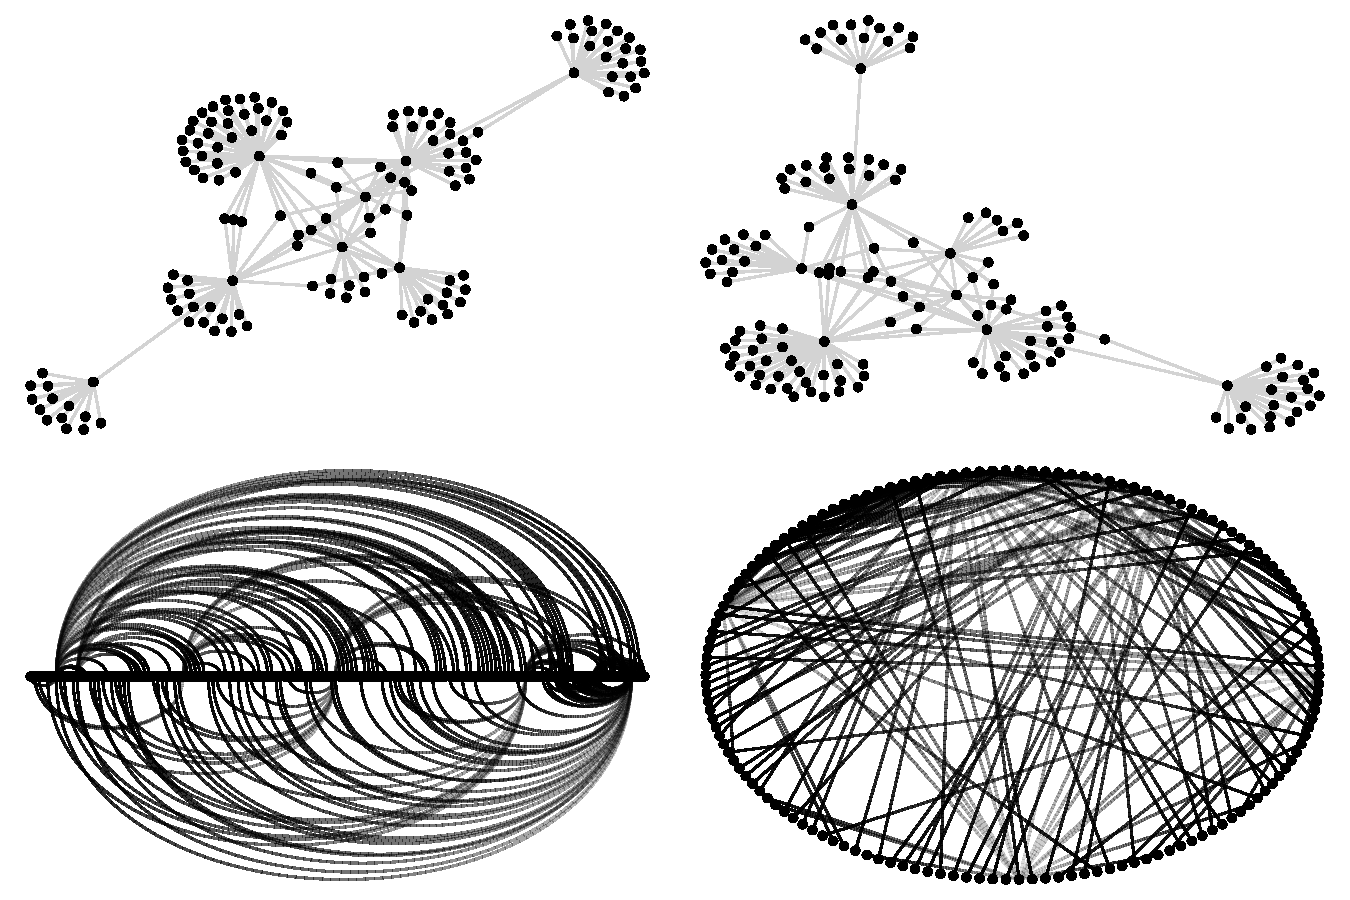
\includegraphics[width=.8\textwidth]{figures/ggraph_vizu_1-1} 

\end{knitrout}
\end{frame}

\begin{frame}
  \frametitle{Layout and Vizualization}
  \framesubtitle{Do not be fooled by the plot}

\begin{knitrout}\scriptsize
\definecolor{shadecolor}{rgb}{0.969, 0.969, 0.969}\color{fgcolor}\begin{kframe}
\begin{alltt}
\hlstd{g.tree} \hlkwb{<-} \hlkwd{graph.formula}\hlstd{(}\hlnum{1}\hlopt{-+}\hlnum{2}\hlstd{,}\hlnum{1}\hlopt{-+}\hlnum{3}\hlstd{,}\hlnum{1}\hlopt{-+}\hlnum{4}\hlstd{,}\hlnum{2}\hlopt{-+}\hlnum{5}\hlstd{,}\hlnum{2}\hlopt{-+}\hlnum{6}\hlstd{,}\hlnum{2}\hlopt{-+}\hlnum{7}\hlstd{,} \hlnum{3}\hlopt{-+}\hlnum{8}\hlstd{,}\hlnum{3}\hlopt{-+}\hlnum{9}\hlstd{,}\hlnum{4}\hlopt{-+}\hlnum{10}\hlstd{)}

\hlkwd{par}\hlstd{(}\hlkwc{mfrow}\hlstd{=}\hlkwd{c}\hlstd{(}\hlnum{1}\hlstd{,} \hlnum{3}\hlstd{))}

\hlkwd{igraph.options}\hlstd{(}\hlkwc{vertex.size}\hlstd{=}\hlnum{30}\hlstd{,} \hlkwc{edge.arrow.size}\hlstd{=}\hlnum{0.5}\hlstd{,} \hlkwc{vertex.label}\hlstd{=}\hlkwa{NULL}\hlstd{)}

\hlkwd{plot}\hlstd{(g.tree,} \hlkwc{layout}\hlstd{=layout.circle)}

\hlkwd{plot}\hlstd{(g.tree,} \hlkwc{layout}\hlstd{=}\hlkwd{layout.reingold.tilford}\hlstd{(g.tree,}  \hlkwc{circular}\hlstd{=T))}

\hlkwd{plot}\hlstd{(g.tree,} \hlkwc{layout}\hlstd{=layout.reingold.tilford)}
\end{alltt}
\end{kframe}
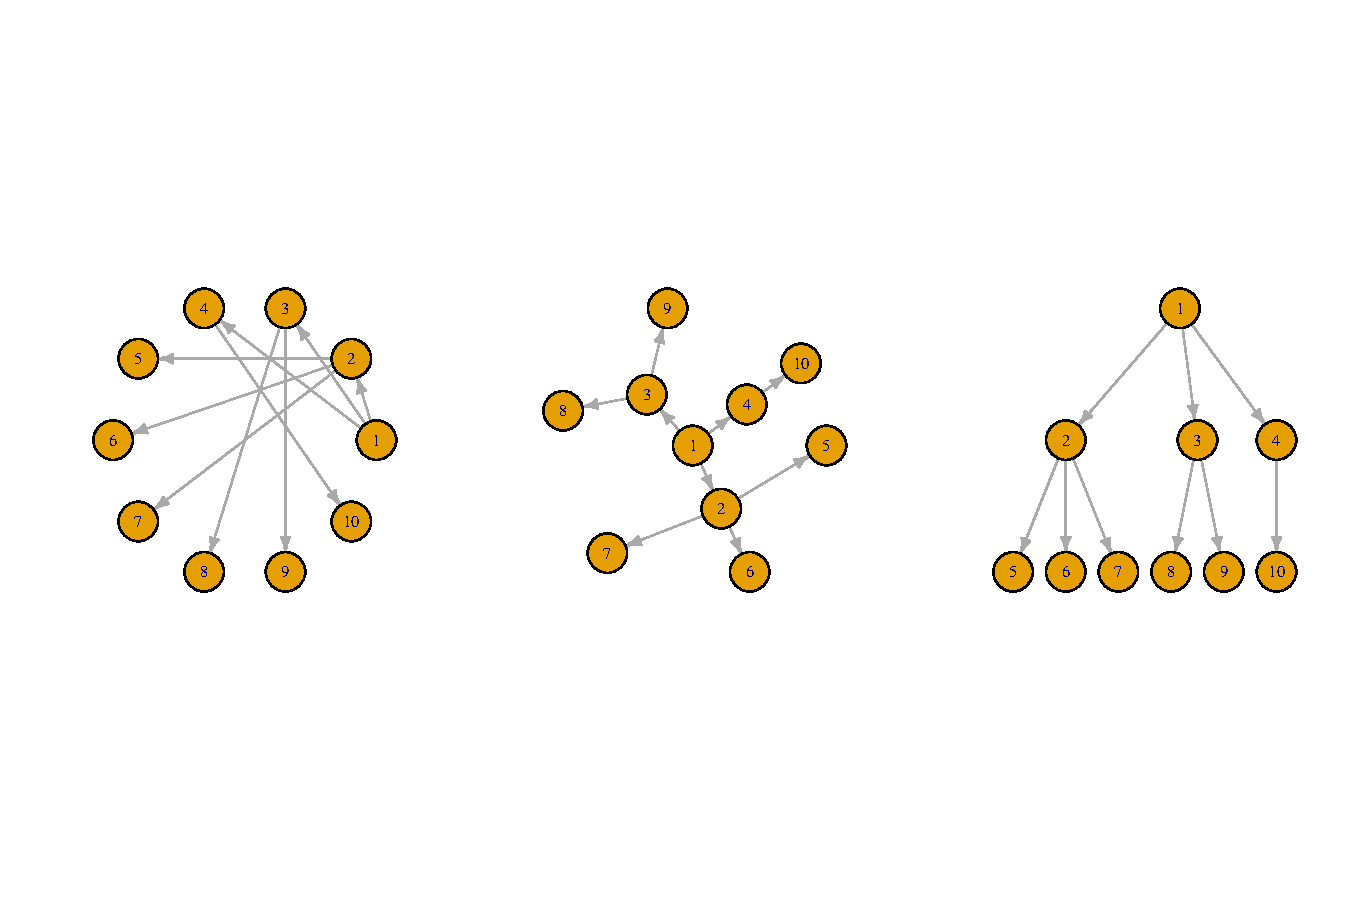
\includegraphics[width=.8\textwidth]{figures/vizu_5-1} 

\end{knitrout}
  
\end{frame}


%% ==========================================================================
\section{Descriptive statistics}
%% ==========================================================================

\begin{frame} 
  \frametitle{References}

    \begin{thebibliography}{99}
      \setbeamertemplate{bibliography item}[book]

    \bibitem[EK2]{EK2} Statistical Analysis of Network Data: Methods and Models, 
    \newblock \textcolor{black}{Eric Kolazcyk}
    \newblock \alert{Chapiter 4, Sections 2 and 3}

    \bibitem[EK1]{EK1} Statistical Analysis of Network Data with \texttt{R}, 
    \newblock \textcolor{black}{Eric Kolazcyk, G\'abor Cs\'ardi}
    \newblock \alert{Chapiter 4, Sections 2 and 3}

      \setbeamertemplate{bibliography item}[article]

    \bibitem[CM1]{CM1} Analyse statistique de graphes, 
    \newblock \textcolor{black}{Catherine Matias}
    \newblock \alert{Chapitre 2}

    \end{thebibliography}

\end{frame}

%% ==========================================================================
\subsection{Vertex characteristics}

\begin{frame}
  \frametitle{Vertex degree}
  
  \begin{definition}[Degree distribution]
    In a graph $\clG = (\clV, \clE)$, recall that $d_i$ counts the number of incident edges in $\clE$ to $i$. Define $f_d$ to be
    the fraction of vertices $i\in \clV$ with degree $d_i=d$. The collection $\set{f_d, d\geq 0}$ is called the \alert{degree distribution} of $\clG$.
  \end{definition}
  
  \begin{block}{Property}
    Many real world networks have a degree distribution fitting well power law distributions: 
    \[
      f_{d_i}(d) = \P(d_i = d) = \frac{c}{d^\gamma}, \quad c\in\Rset, \gamma > 0.
    \]
  \end{block}
  Those heavy-tail distributions describe few vertices with very high degrees.
\end{frame}

\begin{frame}
  \frametitle{Vertex degree: example I}

\begin{knitrout}\scriptsize
\definecolor{shadecolor}{rgb}{0.969, 0.969, 0.969}\color{fgcolor}\begin{kframe}
\begin{alltt}
\hlkwd{library}\hlstd{(sand)}
\hlkwd{data}\hlstd{(karate)}

\hlkwd{par}\hlstd{(}\hlkwc{mfrow}\hlstd{=}\hlkwd{c}\hlstd{(}\hlnum{1}\hlstd{,}\hlnum{2}\hlstd{))}
\hlkwd{plot}\hlstd{(karate)}

\hlkwd{hist}\hlstd{(}\hlkwd{degree}\hlstd{(karate),} \hlkwc{col}\hlstd{=}\hlkwd{adjustcolor}\hlstd{(}\hlstr{"lightblue"}\hlstd{,} \hlkwc{alpha.f} \hlstd{=} \hlnum{0.5}\hlstd{),} \hlkwc{main}\hlstd{=}\hlstr{""}\hlstd{)}
\end{alltt}
\end{kframe}
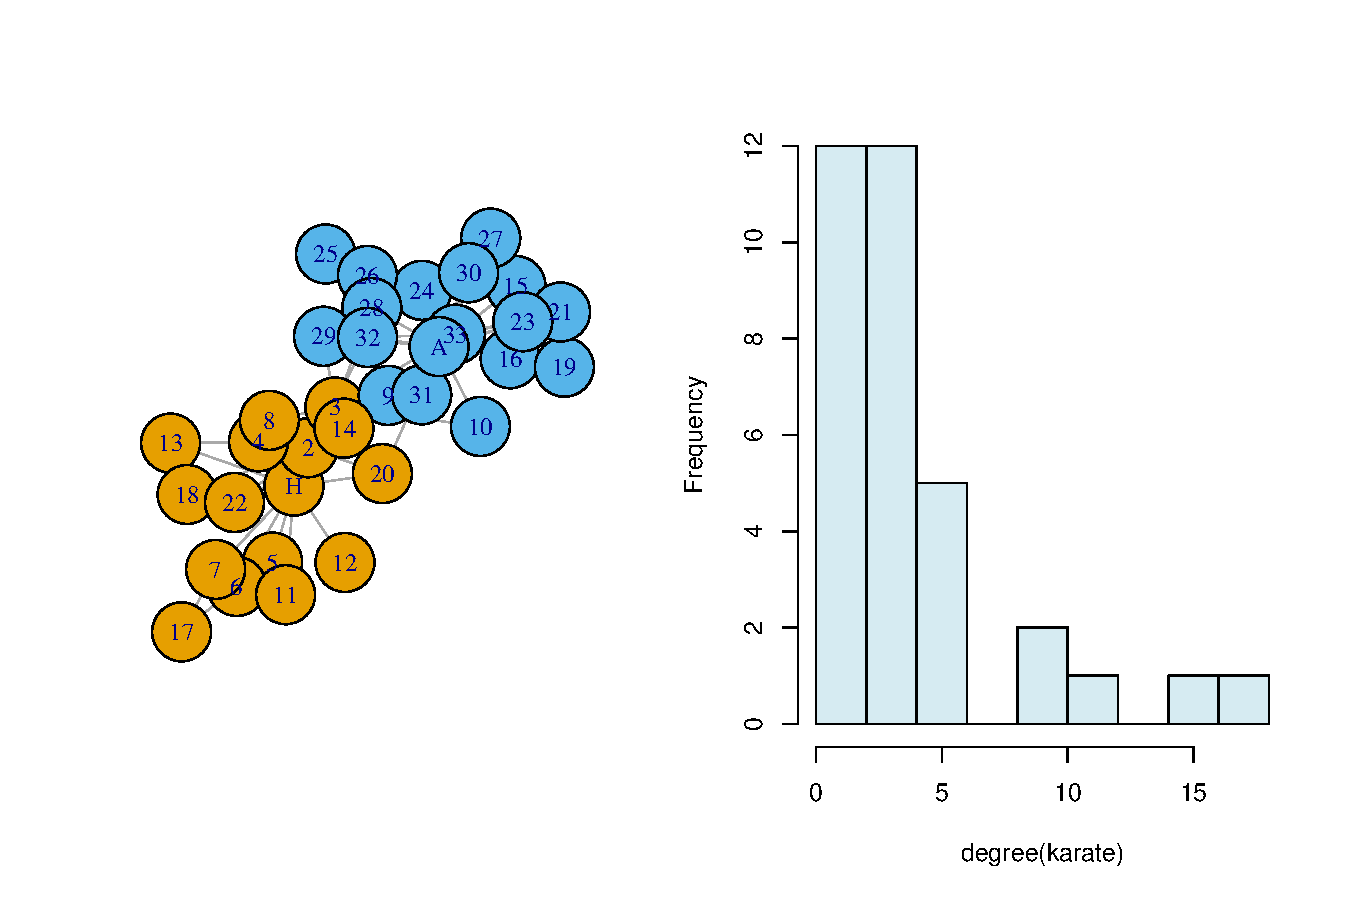
\includegraphics[width=.8\textwidth]{figures/degree_1-1} 

\end{knitrout}
      
\end{frame}

\begin{frame}
  \frametitle{Vertex degree: example II}

\begin{knitrout}\scriptsize
\definecolor{shadecolor}{rgb}{0.969, 0.969, 0.969}\color{fgcolor}\begin{kframe}
\begin{alltt}
\hlkwd{library}\hlstd{(igraphdata)}
\hlkwd{data}\hlstd{(yeast)}

\hlstd{degrees.yeast} \hlkwb{<-} \hlkwd{rev}\hlstd{(}\hlkwd{sort}\hlstd{(}\hlkwd{degree.distribution}\hlstd{(yeast)))}

\hlkwd{plot}\hlstd{(degrees.yeast[degrees.yeast}\hlopt{!=}\hlnum{0}\hlstd{],} \hlkwc{log}\hlstd{=}\hlstr{"xy"}\hlstd{,} \hlkwc{col}\hlstd{=}\hlkwd{adjustcolor}\hlstd{(}\hlstr{"blue"}\hlstd{,} \hlkwc{alpha.f} \hlstd{=} \hlnum{0.5}\hlstd{),} \hlkwc{pch}\hlstd{=}\hlnum{16}\hlstd{,} \hlkwc{xlab}\hlstd{=}\hlstr{"log degree"}\hlstd{,} \hlkwc{ylab}\hlstd{=}\hlstr{"log-intensity"}\hlstd{)}
\end{alltt}
\end{kframe}
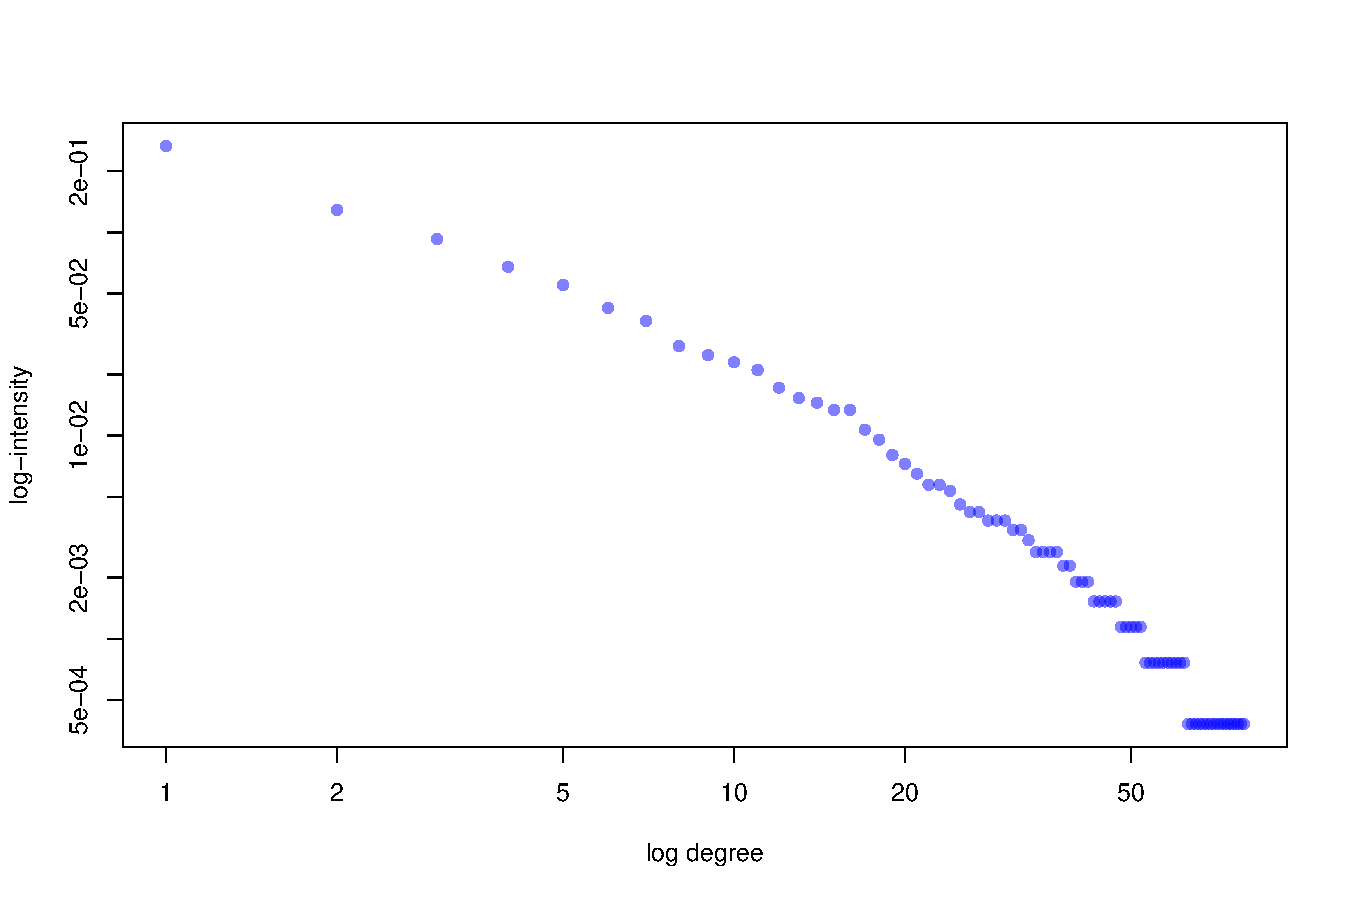
\includegraphics[width=.8\textwidth]{figures/degree_2-1} 

\end{knitrout}
      
\end{frame}

\begin{frame}
  \frametitle{Joint vertex degree distribution}

  \begin{definition}[Empirical distribution of $(d_i, d_j)$]
    Let $\clG = (\clV,\clE$ be an undirected network an let $N(k,\ell)$ be the number of edges whose node have respective degrees equal to $(k,\ell)$ or $(\ell,k)$. Then the empirical distribution of $(d_i,d_j)$ is given by
    \[
      f_{k\ell} = \begin{cases}
      N(k,\ell)/2|\clE| & \text{ if } k < \ell \\
      N(\ell,k)/2|\clE| & \text{ if } k > \ell \\
      N(k,k)/|\clE| & \text{ if } k = \ell \\
      \end{cases}
    \]
  \end{definition}

  \vfill  
  
  \begin{block}{Idea/principle: \textcolor{black}{What kind of nodes share an edge ? }}
    \textit{E.g.} are nodes with high degrees connected with themselves or with low degree vertices?
  \end{block}
  
\end{frame}

\begin{frame}
  \frametitle{Joint degree distribution: example for yeast PPI network}

  \begin{figure}[htbp]
  \centering
  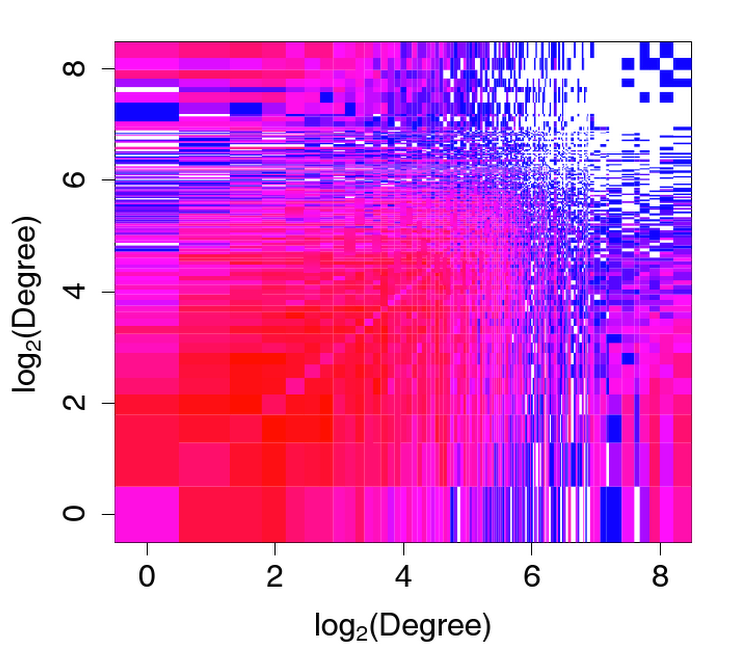
\includegraphics[width=.6\textwidth]{figures/joint_degree_yeast}
  \caption{Image representation of the logarithmically transformed joint degree distribution $\log_2 f_{k\ell}$ of the yeast PPI network (\textit{source}: E. Kolazcyk)}
  \end{figure}
  
\end{frame}

\begin{frame}[allowframebreaks]
  \frametitle{Distance and diameter}

  \begin{definition}[distance]
    \begin{itemize}
    \item \alert{The Length}  of a path $e_1,\dots, e_k$ is the number of edges enterin the path (here $k$).
    \item If two nodes $i,j$ are connected in $G$, then \alert{the distance} $\ell_{ij}$ is the length of the shortest path between $i$ and $j$. If the two nodes are not connected then $\ell_{ij} = \infty$.
    \end{itemize}
  \end{definition}

  \framebreak

  \begin{definition}[mean distance]
    Mean distance in $\clG = (\clV,\clE)$ is defined by
    \[
      \bar{\ell} = \frac{1}{n(n-1)}\sum_{(i,j)\in\clV^2} \ell_{ij} = \frac{2}{n(n-1)}\sum_{i<j} \ell_{ij}.
    \]
  \end{definition}

  \begin{definition}[diameter]
    The diameter of $\clG$ is the greatest distance between two nodes:
    \[
      \mathrm{diameter(\clG)} = \max_{(i,j)\in\clV\times\clV} \left(\ell_{ij}\right)
    \]
  \end{definition}

\end{frame}

\begin{frame}[fragile,allowframebreaks]
  \frametitle{Distance, Diameter: example}
\begin{knitrout}\scriptsize
\definecolor{shadecolor}{rgb}{0.969, 0.969, 0.969}\color{fgcolor}\begin{kframe}
\begin{alltt}
\hlkwd{library}\hlstd{(Matrix)}
\hlkwd{data}\hlstd{(ppi.CC)}
\hlkwd{diameter}\hlstd{(ppi.CC)}
\end{alltt}
\begin{verbatim}
## [1] 12
\end{verbatim}
\begin{alltt}
\hlkwd{average.path.length}\hlstd{(ppi.CC)}
\end{alltt}
\begin{verbatim}
## [1] 4.448039
\end{verbatim}
\begin{alltt}
\hlkwd{image}\hlstd{(}\hlkwd{Matrix}\hlstd{(}\hlkwd{distances}\hlstd{(ppi.CC)))}
\end{alltt}
\end{kframe}
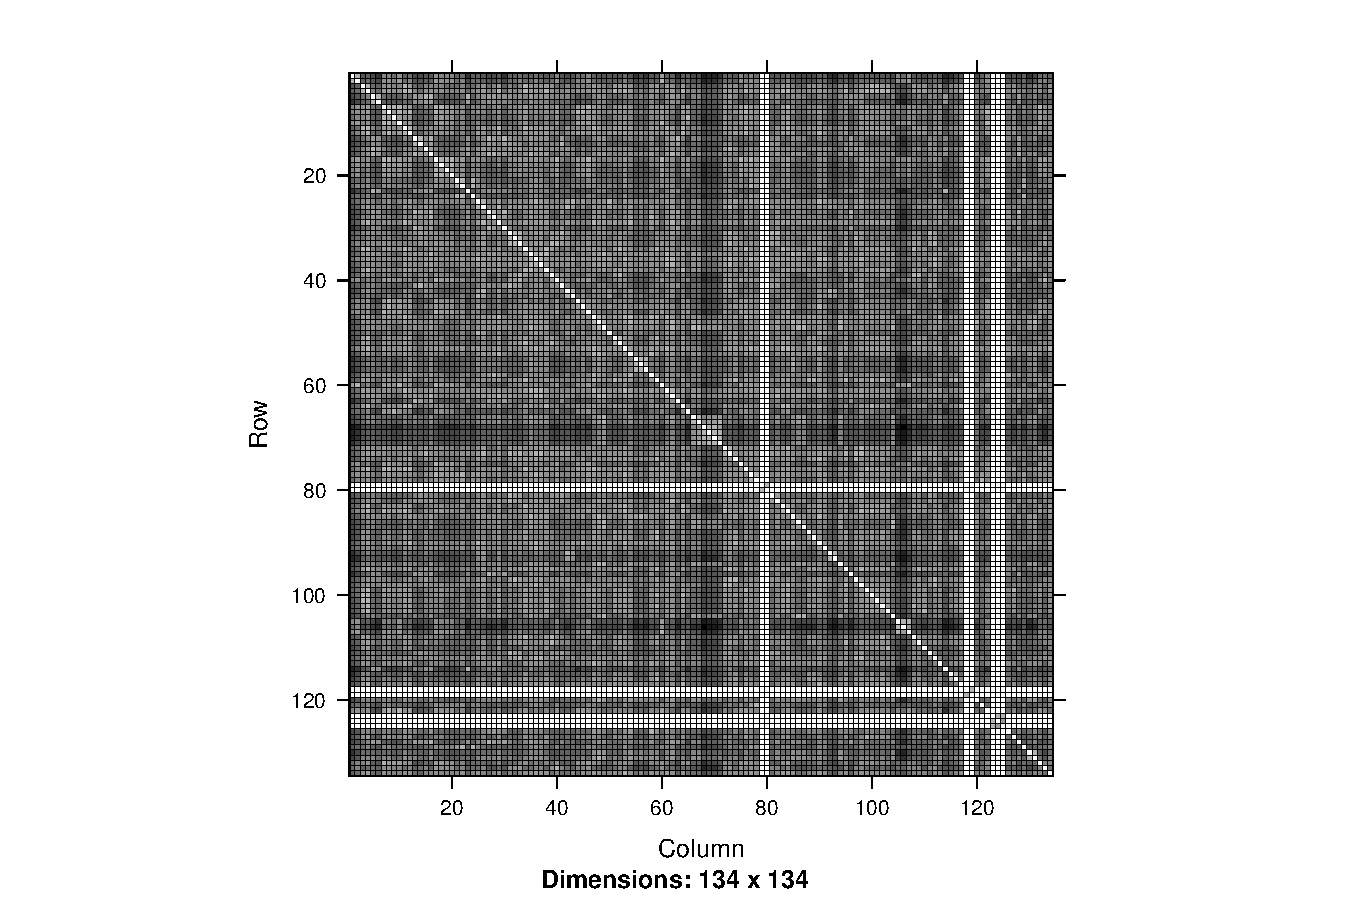
\includegraphics[width=.8\textwidth]{figures/distances1-1} 

\end{knitrout}
\end{frame}

\begin{frame}
  \frametitle{Vertex centrality: closeness}

  \begin{block}{Question}
    How important is the node/vertice in the network?
  \end{block}

  \begin{definition}[Closeness]
    Closeness is the sum of the length of the shortest paths between the node and all other nodes in the graph. It can be defined as the reciprocal of the farness:
    \[C(x)={\frac  {1}{\sum _{y}d(y,x)}}.\]
    $\rightsquigarrow$ \textit{The more central a node is, the closer it is to all other nodes.}
  \end{definition}

\end{frame}

\begin{frame}
  \frametitle{Vertex centrality: betweenness}

  \begin{block}{Question}
    How important is the node/vertice in the network?
  \end{block}

  \begin{definition}[Betweenness]
    For every pairs of vertices, there exists at least one shortest path between the vertices such that the number of edges that the path passes through is minimized.
    The betweenness centrality for each vertex is the number of these shortest paths that pass through the vertex: 
    \[
        g(i)=\sum _{{j\neq i\neq k}}{\frac  {\sigma _{{jk}}(i)}{\sigma _{{jk}}}}    
    \]
    where $\sigma _{jk}$ is the total number of shortest paths from node $j$ to node $k$ and $\sigma _{jk}(i)$ the number of those paths that pass through $i$.

  \end{definition}

\end{frame}

\begin{frame}[fragile]
  \frametitle{Example for karate club data set}
  \framesubtitle{administrator and instructor are in blue and yellow}

\begin{knitrout}\scriptsize
\definecolor{shadecolor}{rgb}{0.969, 0.969, 0.969}\color{fgcolor}
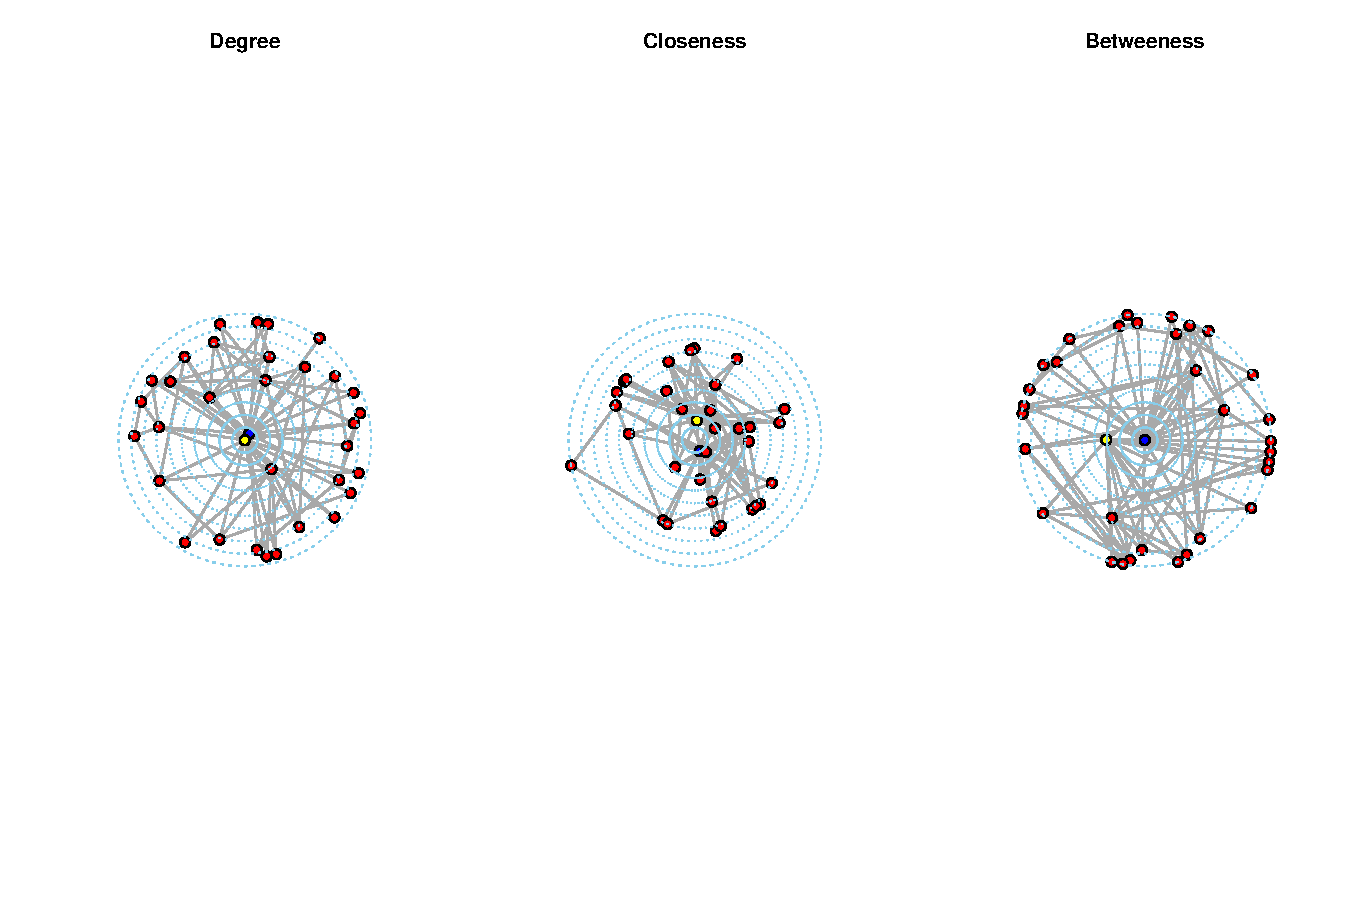
\includegraphics[width=\textwidth]{figures/density-1} 

\end{knitrout}

\end{frame}

\begin{frame}
  \frametitle{Jaccard Coefficient}

  \begin{definition}[Jaccard Coefficient or Jaccard Index]
The Jaccard coefficient \alert{measures similarity between finite sample sets}, and is defined as the size of the intersection divided by the size of the union of the sample sets:
  \[
  J(A,B)=\frac{|A\cap B|}{|A\cup B|} =\frac{|A\cap B|}{|A|+|B|-|A\cap B|}.
  \]
  \end{definition}

  \begin{block}{Example}
  It can be used to compared two sets of egdes. For instance
  \begin{itemize}
    \item for two networks $\clG$ and $\clH$ defined on the same set of node, we can compare the sets $\clE_\clG$ and $\clE_\clH$.
    \item for a networks $\clG$ we can compute similarity between nodes with the Jaccard index and use it to define a weighted graph of similarity.
  \end{itemize}
  \end{block}

\end{frame}

\begin{frame}[fragile]
  \frametitle{Jaccard Coefficient: example}

Plot the yeast PPI interaction network
\begin{knitrout}\scriptsize
\definecolor{shadecolor}{rgb}{0.969, 0.969, 0.969}\color{fgcolor}\begin{kframe}
\begin{alltt}
\hlkwd{library}\hlstd{(sand)}
\hlkwd{library}\hlstd{(igraph)}
\hlkwd{plot}\hlstd{(ppi.CC,} \hlkwc{vertex.size}\hlstd{=}\hlnum{6}\hlstd{,} \hlkwc{vertex.label}\hlstd{=}\hlnum{NA}\hlstd{,} \hlkwc{layout}\hlstd{=layout_in_circle)}
\end{alltt}
\end{kframe}
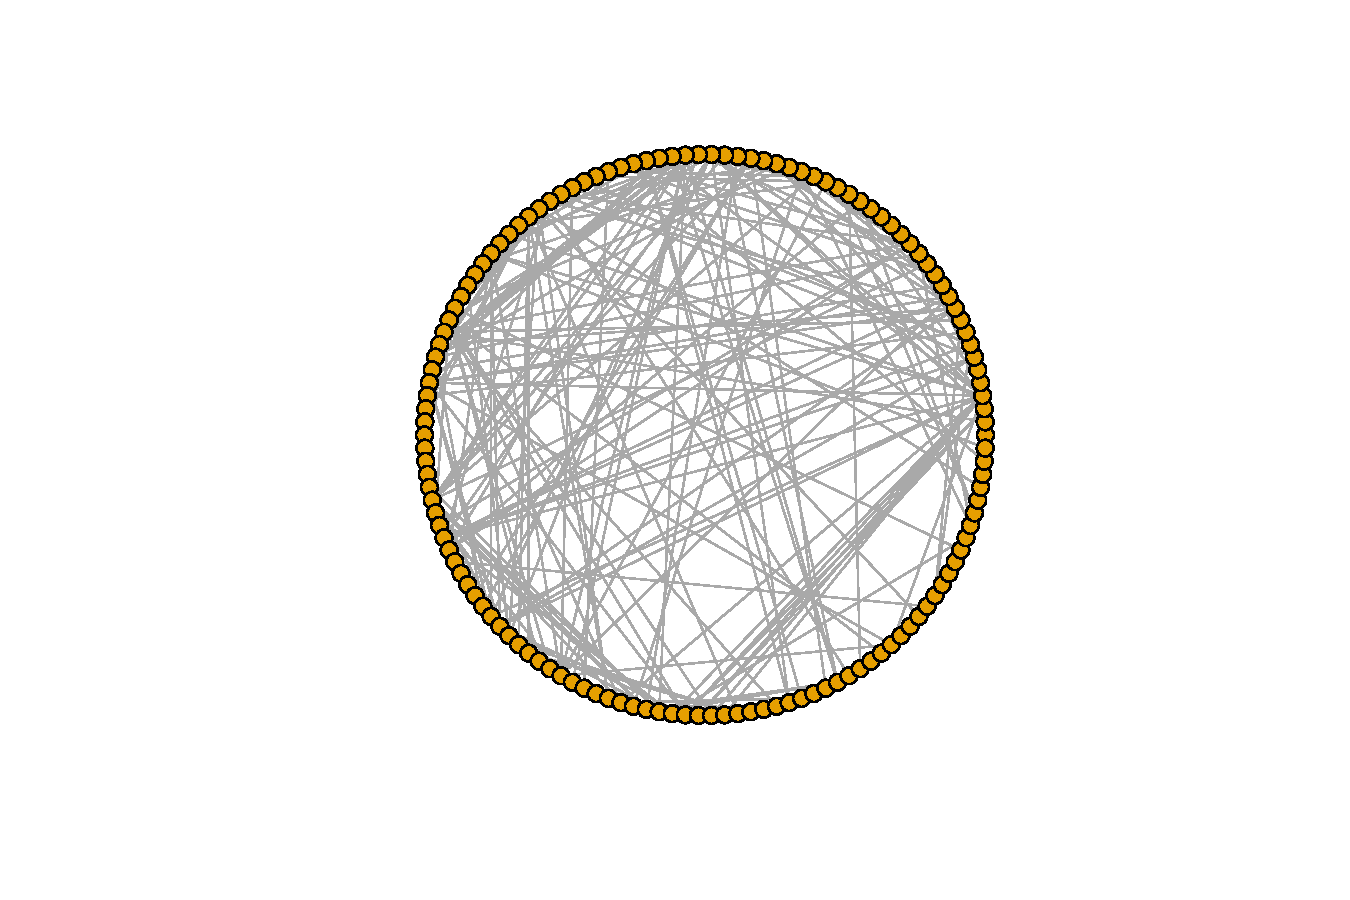
\includegraphics[width=.8\textwidth]{figures/jaccard-1} 

\end{knitrout}

\end{frame}

\begin{frame}[fragile]
  \frametitle{Jaccard Coefficient: example II}

Compute Jaccard similarity between vertices and give a image of this
\begin{knitrout}\scriptsize
\definecolor{shadecolor}{rgb}{0.969, 0.969, 0.969}\color{fgcolor}\begin{kframe}
\begin{alltt}
\hlkwd{library}\hlstd{(Matrix)}
\hlkwd{image}\hlstd{(}\hlkwd{Matrix}\hlstd{(igraph}\hlopt{::}\hlkwd{similarity}\hlstd{(ppi.CC,} \hlkwc{method} \hlstd{=} \hlstr{"jaccard"}\hlstd{)))}
\end{alltt}
\end{kframe}
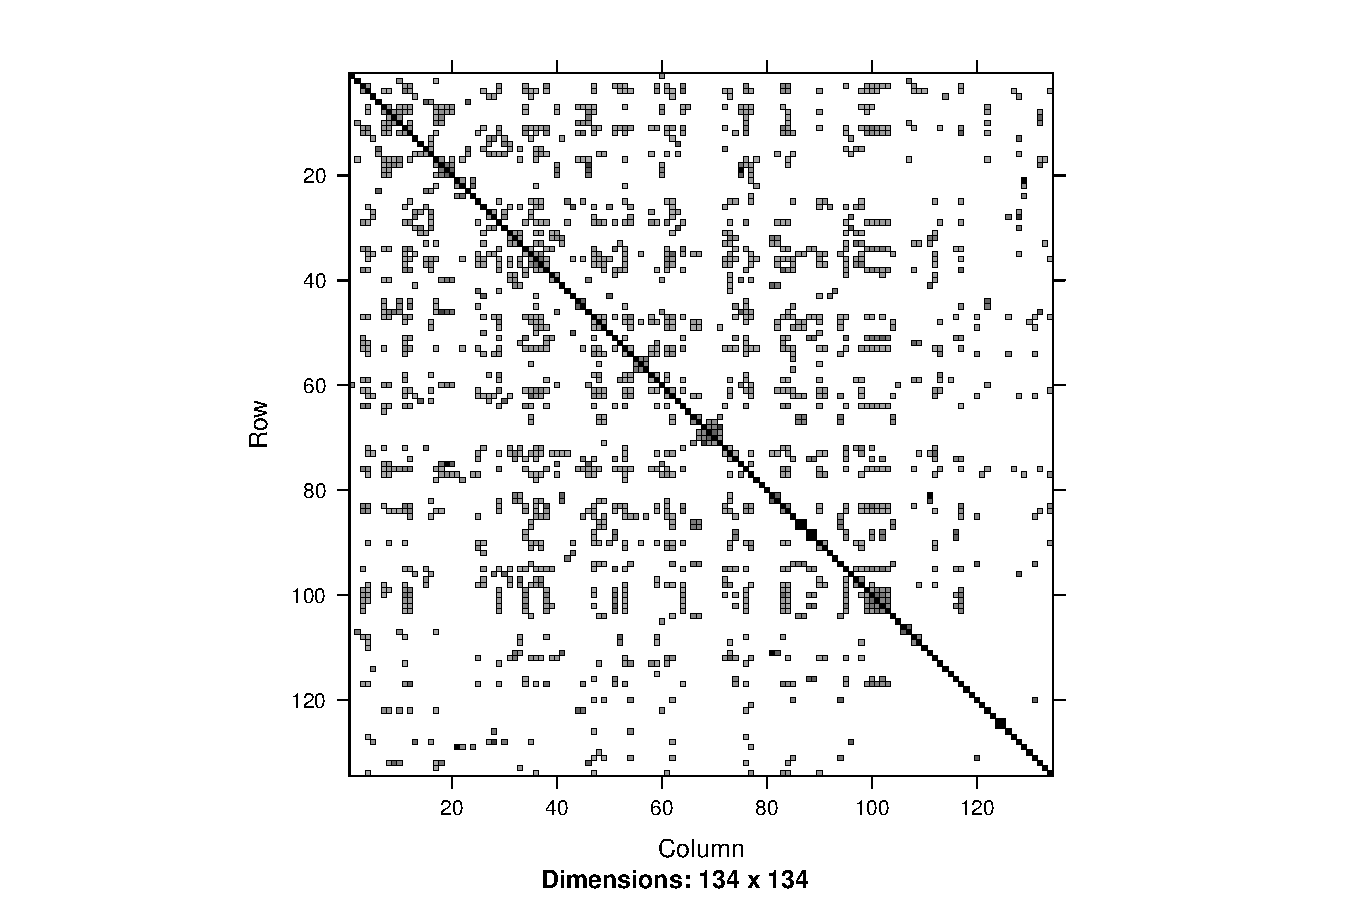
\includegraphics[width=.8\textwidth]{figures/jaccardplot-1} 

\end{knitrout}

\end{frame}

%% ==========================================================================
\subsection{Local measurements}

\begin{frame}
  \frametitle{Density}

  \begin{block}{Question}
    Is the network locally \alert{dense} in some sense?
  \end{block}

  \begin{definition}[Clique]
    In an undirected graph, a clique is a subset of the vertices such that \alert{every two distinct vertices are adjacent}.
  \end{definition}


  \begin{definition}[Density]
    The density of a (sub)-graph $\clG = (\clV,\clE)$ is defined by
    \[
      \mathrm{density}(\clG) = \frac{2|\clE|}{|\clV|(|\clV| - 1)} = \frac{\bar{D}}{|V|-1},
    \]
    where $\bar{D}$ is the mean degree of the network: how much $\clG$ is close to a clique? 
  \end{definition}

\end{frame}

\begin{frame}
  \frametitle{Clustering}

  \begin{block}{Question}
    Is the network locally \alert{dense} in some sense?
  \end{block}

  \begin{definition}[Triangle]
    Triplets of vertices in the graph that are connected through a triangle. They correspond to transitive relationships. We let 
    \begin{itemize}
      \item $\tau_{\Delta}(i)$ be the number of triangles in $\clG$ where $i$ falls.
      \item $\tau_{3}(i)$ be the number of triplets in $\clG$ where $i$ falls.
    \end{itemize}    
  \end{definition}


  \begin{definition}[Clustering coefficient]
    \[
      \mathrm{clustering}(\clG) = \frac{1}{\clV_2} \sum_{i\in\clV_2} \tau_{\Delta}(i) / \tau_3(i),
    \]
    where $\clV_2$ is the set of vertices whose degree is greater or equal to 2.
  \end{definition}

\end{frame}

\begin{frame}
  \frametitle{Transitivity}

  \begin{block}{Question}
    Is the network locally \alert{dense} in some sense?
  \end{block}

  \begin{definition}[Triangle]
    Triplet of vertices in the graph that are connected through a triangle. They correspond to transitive relationships. We let 
    \begin{itemize}
      \item $\tau_{\Delta}(i)$ be the number of triangle in $\clG$ where $i$ falls.
      \item $\tau_{3}(i)$ be the number of triplet in $\clG$ where $i$ falls.
    \end{itemize}    
  \end{definition}

  \begin{definition}[Transitivity]
    
    \[
      \mathrm{transitivity}(\clG) = \frac{\sum_{\clV}\tau_{\Delta}(i)}{\sum_{\clV}\tau_3(i)},
    \]
  \end{definition}

\end{frame}

\begin{frame}
  \frametitle{Motifs}

  \begin{block}{Question}
    Is the network locally \alert{dense} in some sense?
  \end{block}

  $\rightsquigarrow$ This question can be ansered thank to more complicated motifs than cliques and triangles\dots
\end{frame}


\begin{frame}[fragile]
  \frametitle{Local density: example}



Create ego graphs around teacher and instructor
\begin{knitrout}\scriptsize
\definecolor{shadecolor}{rgb}{0.969, 0.969, 0.969}\color{fgcolor}\begin{kframe}
\begin{alltt}
\hlkwd{data}\hlstd{(karate)}

\hlstd{ego.instr} \hlkwb{<-} \hlkwd{induced.subgraph}\hlstd{(karate,} \hlkwd{neighborhood}\hlstd{(karate,} \hlnum{1}\hlstd{,} \hlnum{1}\hlstd{)[[}\hlnum{1}\hlstd{]])}
\end{alltt}


{\ttfamily\noindent\bfseries\color{errorcolor}{\#\# Error in FUN(X[[i]], ...): as.sociomatrix.sna input must be an adjacency matrix/array, network, or list.}}\begin{alltt}
\hlstd{ego.admin} \hlkwb{<-} \hlkwd{induced.subgraph}\hlstd{(karate,} \hlkwd{neighborhood}\hlstd{(karate,} \hlnum{1}\hlstd{,} \hlnum{34}\hlstd{)[[}\hlnum{1}\hlstd{]])}
\end{alltt}


{\ttfamily\noindent\bfseries\color{errorcolor}{\#\# Error in FUN(X[[i]], ...): as.sociomatrix.sna input must be an adjacency matrix/array, network, or list.}}\end{kframe}
\end{knitrout}

\begin{knitrout}\scriptsize
\definecolor{shadecolor}{rgb}{0.969, 0.969, 0.969}\color{fgcolor}\begin{kframe}


{\ttfamily\noindent\bfseries\color{errorcolor}{\#\# Error in plot(ego.instr): object 'ego.instr' not found}}

{\ttfamily\noindent\bfseries\color{errorcolor}{\#\# Error in plot(ego.admin): object 'ego.admin' not found}}\end{kframe}
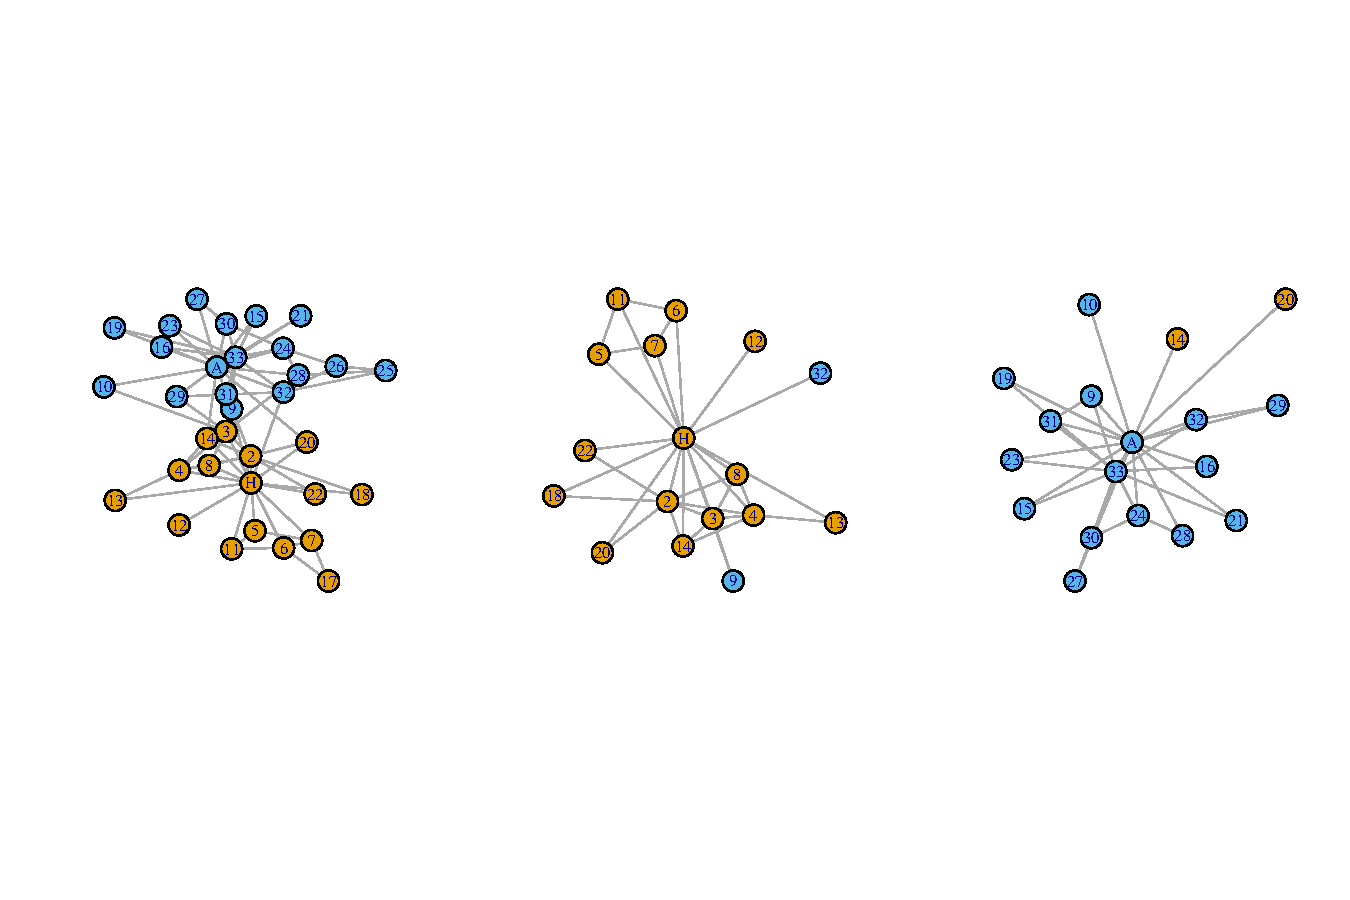
\includegraphics[width=.8\textwidth]{figures/density3-1} 

\end{knitrout}

\end{frame}

\begin{frame}[fragile]
  \frametitle{Local density: example II}

Maximal clique size, number of triangle
\begin{knitrout}\scriptsize
\definecolor{shadecolor}{rgb}{0.969, 0.969, 0.969}\color{fgcolor}\begin{kframe}
\begin{alltt}
\hlkwd{clique.number}\hlstd{(karate)}
\end{alltt}
\begin{verbatim}
## [1] 5
\end{verbatim}
\begin{alltt}
\hlkwd{clique.number}\hlstd{(ego.admin)}
\end{alltt}


{\ttfamily\noindent\bfseries\color{errorcolor}{\#\# Error in "{}igraph"{} \%in\% class(graph): object 'ego.admin' not found}}\begin{alltt}
\hlkwd{length}\hlstd{(}\hlkwd{triangles}\hlstd{(karate))}
\end{alltt}
\begin{verbatim}
## [1] 135
\end{verbatim}
\begin{alltt}
\hlkwd{length}\hlstd{(}\hlkwd{triangles}\hlstd{(ego.admin))}
\end{alltt}


{\ttfamily\noindent\bfseries\color{errorcolor}{\#\# Error in "{}igraph"{} \%in\% class(graph): object 'ego.admin' not found}}\end{kframe}
\end{knitrout}

\end{frame}

\begin{frame}[fragile]
  \frametitle{Local density: example III}

Efficient motif counts
\begin{knitrout}\scriptsize
\definecolor{shadecolor}{rgb}{0.969, 0.969, 0.969}\color{fgcolor}\begin{kframe}
\begin{alltt}
\hlkwd{cliques}\hlstd{(karate,} \hlkwc{min} \hlstd{=} \hlnum{5}\hlstd{)}
\end{alltt}
\begin{verbatim}
## [[1]]
## + 5/34 vertices, named, from 4b458a1:
## [1] Mr Hi    Actor 2  Actor 3  Actor 4  Actor 14
## 
## [[2]]
## + 5/34 vertices, named, from 4b458a1:
## [1] Mr Hi   Actor 2 Actor 3 Actor 4 Actor 8
\end{verbatim}
\begin{alltt}
\hlkwd{count_triangles}\hlstd{(karate)}
\end{alltt}
\begin{verbatim}
##  [1] 18 12 11 10  2  3  3  6  5  0  2  0  1  6  1  1  1  1  1  1  1  1  1
## [24]  4  1  1  1  1  1  4  3  3 13 15
\end{verbatim}
\end{kframe}
\end{knitrout}

\end{frame}

\begin{frame}[fragile]
  \frametitle{Local density: example IV}

Look for graph density and transitivity/clustering either globally or locally
\begin{knitrout}\scriptsize
\definecolor{shadecolor}{rgb}{0.969, 0.969, 0.969}\color{fgcolor}\begin{kframe}
\begin{alltt}
\hlkwd{graph.density}\hlstd{(karate)}
\end{alltt}
\begin{verbatim}
## [1] 0.1390374
\end{verbatim}
\begin{alltt}
\hlkwd{graph.density}\hlstd{(ego.instr)}
\end{alltt}


{\ttfamily\noindent\bfseries\color{errorcolor}{\#\# Error in "{}igraph"{} \%in\% class(graph): object 'ego.instr' not found}}\begin{alltt}
\hlkwd{graph.density}\hlstd{(ego.admin)}
\end{alltt}


{\ttfamily\noindent\bfseries\color{errorcolor}{\#\# Error in "{}igraph"{} \%in\% class(graph): object 'ego.admin' not found}}\begin{alltt}
\hlkwd{transitivity}\hlstd{(karate)}
\end{alltt}
\begin{verbatim}
## [1] 0.2556818
\end{verbatim}
\begin{alltt}
\hlkwd{transitivity}\hlstd{(karate,} \hlstr{"local"}\hlstd{,} \hlkwc{vids}\hlstd{=}\hlkwd{c}\hlstd{(}\hlnum{1}\hlstd{,}\hlnum{34}\hlstd{))}
\end{alltt}
\begin{verbatim}
## [1] 0.1500000 0.1102941
\end{verbatim}
\end{kframe}
\end{knitrout}

\end{frame}


%% ==========================================================================
\section{Graph Partionning}
%% ==========================================================================

\begin{frame} 
  \frametitle{References}

    \begin{thebibliography}{99}
      \setbeamertemplate{bibliography item}[book]

    \bibitem[EK2]{EK2} Statistical Analysis of Network Data: Methods and Models,
    \newblock \textcolor{black}{Eric Kolazcyk}
    \newblock \alert{Chapiter 4, Section 4}

    \bibitem[EK1]{EK1} Statistical Analysis of Network Data with \texttt{R}, 
    \newblock \textcolor{black}{Eric Kolazcyk, G\'abor Cs\'ardi}
    \newblock \alert{Chapiter 4, Section 4}

      \setbeamertemplate{bibliography item}[article]

    \bibitem[CM1]{CM1} Analyse statistique de graphes, 
    \newblock \textcolor{black}{Catherine Matias}
    \newblock \alert{Chapitre 3}
    
    \bibitem[VLB]{VLB} A Tutorial on Spectral Clustering, 
    \newblock \textcolor{black}{Ulrike von Luxburg}

    \end{thebibliography}

\end{frame}

\begin{frame}
  \frametitle{Principle of graph partionning}

  \begin{definition}[Partition]
    A decomposition $\mathcal{C} = \{C_1,\dots,C_K\}$ of the vertices $\clV$ such that
    \begin{itemize}
      \item $C_k \cap C_{k'} = \emptyset$ for any $k\neq k'$
      \item $\bigcup_{k} C_k = \clV$
    \end{itemize}
  \end{definition}

  \vfill

  \begin{block}{Goal of graph paritionning}
    Form a partition of the vertices with unsupervized approach where the $\mathcal{C}$ is composed by \alert{"cohesive"} sets of vertices, for instance,
    \begin{enumerate}
      \item vertices well connected among themselves
      \item well separated from the remaining vertices
    \end{enumerate}
    
  \end{block}

\end{frame}

%% ==========================================================================
\subsection{Hierarchical clustering}

\begin{frame}
  \frametitle{Principle}
  \framesubtitle{}


  \begin{algorithm}[H]
    \KwIn{$n$ individuals with $p$ attributes)}
    \BlankLine\BlankLine
    \DontPrintSemicolon
      1. Compute the dissimilarity between groups \;
      2. Regroup the two most similar elements \;
      
      Iterate until all element are in a single group \;
    \BlankLine\BlankLine
    \KwOut{$n$ nested partitions from $\set{\set{1},\dots,\set{n}}$ to $\set{\set{1,\dots,n}}$}

    \caption{Agglomerative hierarchical clustering}
  \end{algorithm}
  
  \begin{block}{Ingredients}
    \begin{enumerate}
      \item a dissimilarity measure between singleton
      \item a distance measure between sets
    \end{enumerate}
  \end{block}

\end{frame}

\begin{frame}
  \frametitle{Dissimilarity measures}

  \begin{block}{Standards}
    Use standard distances on adjacency matrix:
    \begin{itemize}
      \item Euclidean distance: $\displaystyle x_{ij} = \sqrt{\sum_{ij} (A_{ik} - A_{jk})^2} $
      \item Manhattan distance: $\displaystyle x_{ij} = \sum_{ij} |A_{ik} - A_{jk})^2| $
      \item  etc\dots
    \end{itemize}  
  \end{block}

  \vfill

  \begin{block}{Graph-specific}
    For instance,  Modularity (studied during tutorial)
  \end{block}
  
\end{frame}

\begin{frame}[fragile,allowframebreaks]
  \frametitle{Examples of graph clustering}

\begin{knitrout}\scriptsize
\definecolor{shadecolor}{rgb}{0.969, 0.969, 0.969}\color{fgcolor}\begin{kframe}
\begin{alltt}
\hlstd{hc} \hlkwb{<-} \hlkwd{cluster_fast_greedy}\hlstd{(karate)}
\hlkwd{plot}\hlstd{(hc,karate)}
\end{alltt}
\end{kframe}
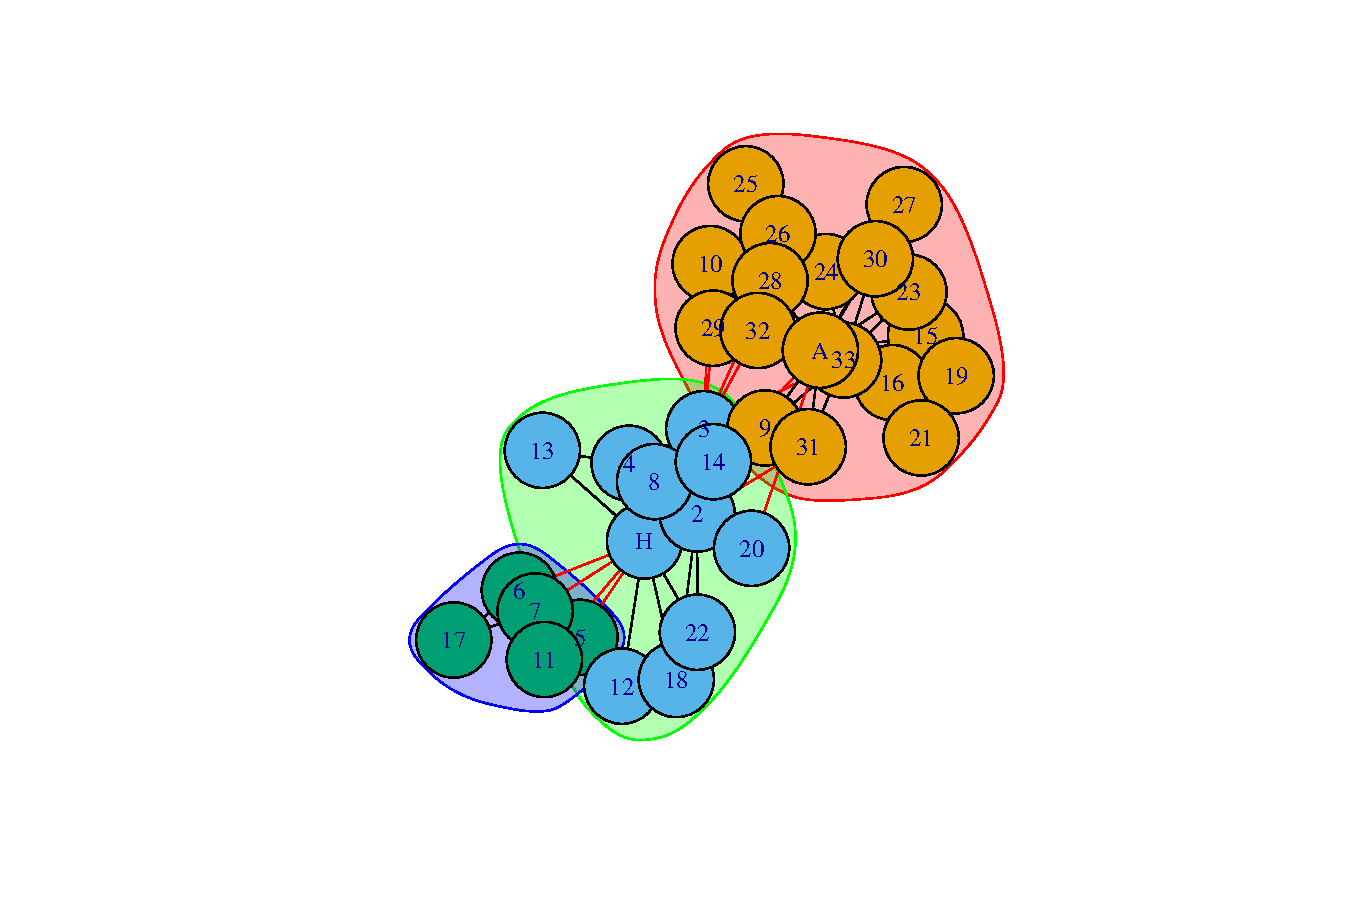
\includegraphics[width=.8\textwidth]{figures/unnamed-chunk-2-1} 

\end{knitrout}

\begin{knitrout}\scriptsize
\definecolor{shadecolor}{rgb}{0.969, 0.969, 0.969}\color{fgcolor}\begin{kframe}
\begin{alltt}
\hlstd{hc} \hlkwb{<-} \hlkwd{cluster_edge_betweenness}\hlstd{(karate)}
\hlkwd{plot}\hlstd{(hc,karate)}
\end{alltt}
\end{kframe}
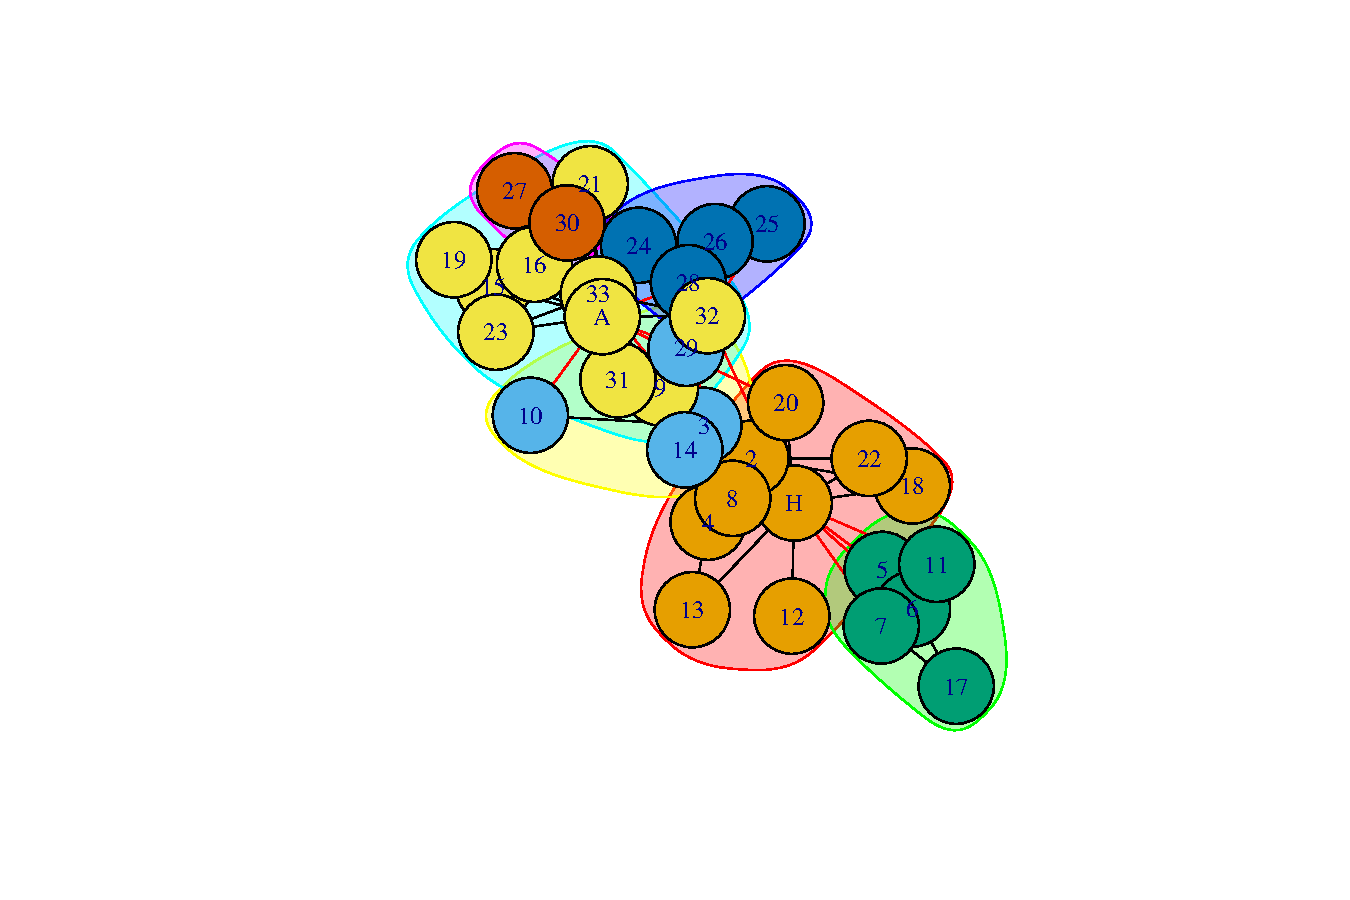
\includegraphics[width=.8\textwidth]{figures/unnamed-chunk-3-1} 

\end{knitrout}

\begin{knitrout}\scriptsize
\definecolor{shadecolor}{rgb}{0.969, 0.969, 0.969}\color{fgcolor}\begin{kframe}
\begin{alltt}
\hlstd{hc} \hlkwb{<-} \hlkwd{cluster_walktrap}\hlstd{(karate)}
\hlkwd{plot}\hlstd{(hc,karate)}
\end{alltt}
\end{kframe}
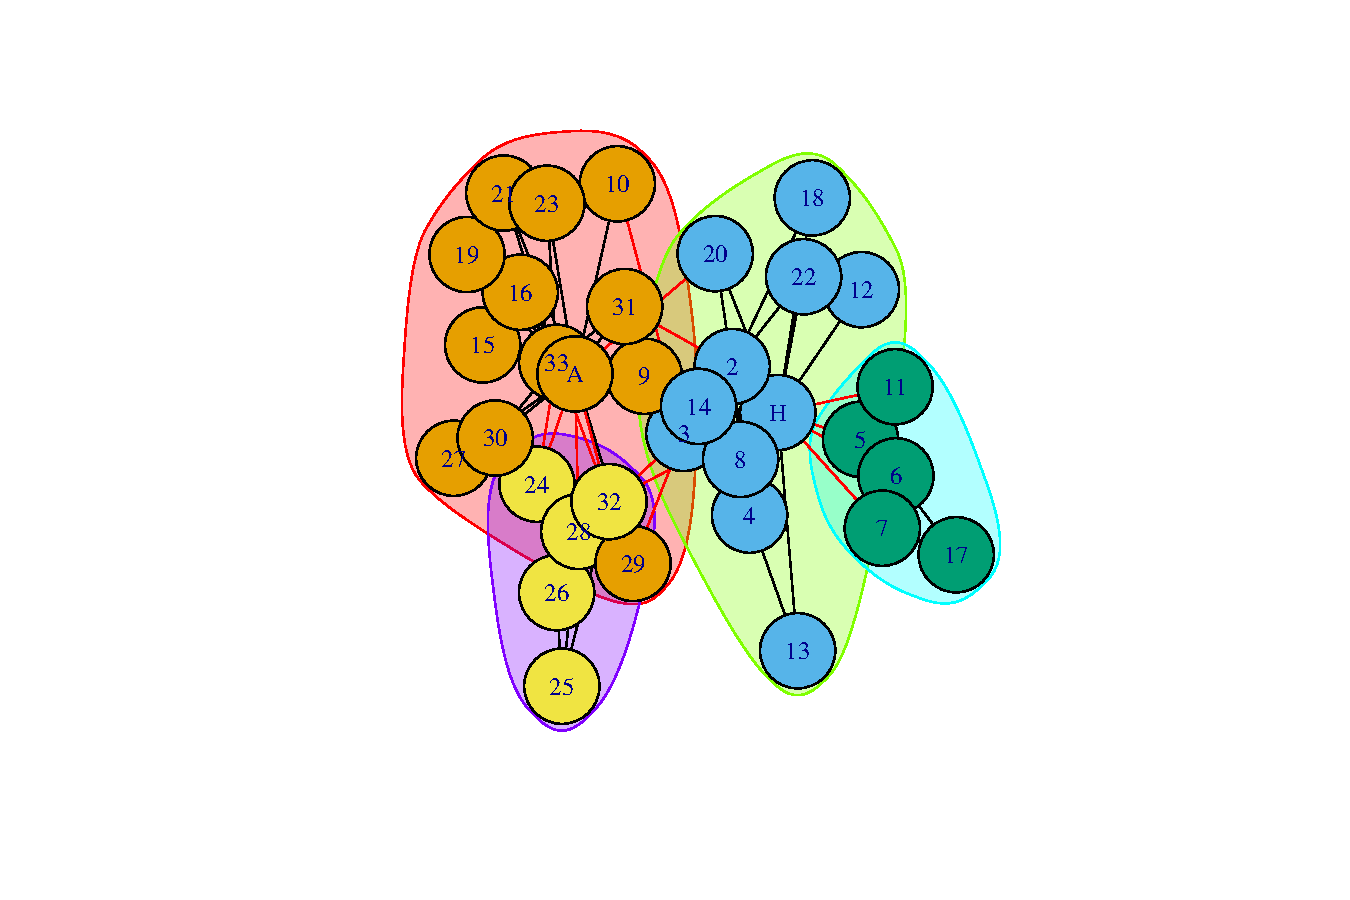
\includegraphics[width=.8\textwidth]{figures/unnamed-chunk-4-1} 

\end{knitrout}

\end{frame}

%% ==========================================================================
\subsection{Spectral Clustering}

\begin{frame}
  \frametitle{Graph Laplacian}

  \begin{definition}[(Un-normalized) Laplacian]
    The Laplacian matrix $\bL$, resulting from the modified incidence matrix $\tilde\bB$ $\tilde{\! B}_{ij}= 1/-1$ if $i$ is incident to $j$ as tail/head, is defined by 
    \[
      \bL = \tilde \bB \tilde \bB^\intercal = \bD - \bA,
    \]
    where $\bD = \diag(d_i, i\in\clV)$ is the diagonal matrix of degrees. 
  \end{definition}

  \begin{block}{Remark}
    \begin{itemize}
    \item $\bL$ is called Laplacian by analogy to the second order derivative (see below).
    \item Spectrum of $\bL$ has much to say about the structure of the graph $\clG$.
    \end{itemize}
  \end{block}

\end{frame}

\begin{frame}
  \frametitle{Graph Laplacian: spectrum}

  \begin{proposition}[Spectrum of $\bL$]
    The $n\times n$ matrix $\bL$ has the following properties:
    \[
      \bx^\top \bL \bx = \frac{1}{2} \sum_{i,j} A_{ij} (x_i - x_j)^2, \quad \forall \bx\in\Rset^n .
    \]
    \vspace{-.25cm}
    \begin{itemize}
      \item $\bL$ is a symmetric, positive semi-definite matrix,
      \item  the smallest eigenvalue is $0$ with associated eigenvector $\mathbf{1}$.K
      \item $\bL$ has $n$ positive eigenvalues $0=\lambda_1<\dots <\lambda_n$. 
    \end{itemize}  
  \end{proposition}

  \begin{corollary}[Spectrum and Graph]
    \vspace{-.25cm}
    \begin{itemize}
      \item The multiplicity of the first eigen value ($0$) of $\bL$ determines the number of connected components in the graph.
      \item The larger the second non trivial eigenvalue, the higher the connectivity of $\clG$.
    \end{itemize}  
  \end{corollary}

\end{frame}

\begin{frame}
  \frametitle{Normalized Graph Laplacian}

  \begin{definition}[(Normalized) Laplacian]
    The normalized Laplacian matrix $\bL$ is defined by 
    \[
      \bL_N = \bD^{-1/2}\bL\bD^{-1/2} = \bI - \bD^{-1/2} \bA \bD^{-1/2}.
    \]
  \end{definition}

  \begin{proposition}
    The $n\times n$ matrix $\bL_N$ has the following properties:
      \[
        \bx^\top \bL_N \bx = \frac{1}{2} \sum_{i,j} A_{ij}\left(\frac{x_i}{\sqrt{d_i}} - \frac{x_j}{\sqrt{d_j}} \right)^2, quad\forall\bx\in\Rset^n.
      \]
    \vspace{-.25cm}
    \begin{itemize}
      \item $\bL$ is a symmetric, positive semi-definite matrix, with $n$ nonnegative eigenvalues $0=\lambda_1<\dots <\lambda_n$
      \item  the smallest eigenvalue is $0$ with associated eigenvector $\bD^{-1/2}\mathbf{1}$.
    \end{itemize}  
  \end{proposition}

\end{frame}

\begin{frame}
  \frametitle{Absolute Graph Laplacian}

  \begin{definition}[(Absolute) Laplacian]
    The absolute Laplacian matrix $\bL_{abs}$ is defined by 
    \[
      \bL_{abs} = \bD^{-1/2}\bA\bD^{-1/2} = \bI - \bL_N,
    \]
    with eigenvalues $1-\lambda_n \leq \dots \leq 1-\lambda_2 \leq 1-\lambda_1 = 1$, where $0=\lambda_1\leq \dots \leq \lambda_n$ are the eigenvalues of $\bL_N$.
  \end{definition}

\end{frame}

\begin{frame}
  \frametitle{Spectral Clustering}
    
  \begin{block}{Principle}
  
  \begin{enumerate}
    \item Use the spectral property of $\bL$ to perform clustering in the eigen space \medskip
    \item If the network have $K$ connected components, the first $K$ eigenvectors are $\mathbf{1}$ span the eigenspace associated with eigenvalue $0$ \medskip
    \item Applying a simple clustering algorithm to the rows of the $K$ first eigenvectors separate the components
  \end{enumerate}
  $\rightsquigarrow$ This principle generalizes to a graph with a single component: spectral clustering tends to separates groups of nodes which are highly connected together
  
  \end{block}
  
\end{frame}

\begin{frame}
  \frametitle{Normalized Spectral Clustering}

\begin{algorithm}[H]
  \KwIn{Adjacency matrix and number of classes $Q$}
  \BlankLine\BlankLine
  \DontPrintSemicolon
  
  Compute the normalized graph Laplacian $\mathbf{L}$\;
  Compute the eigen vectors of $\mathbf{L}$ associated with the $Q$ \alert{smallest eigenvalues}\;
  Define $\mathbf{U}$,  the $p\times Q$ matrix  that encompasses these $Q$ vectors \;
  Define $\tilde{\mathbf{U}}$, the row-wise normalized version of $\mathbf{U}$: $ \tilde{u}_{ij} = \frac{u_{ij}}{\| \mathbf{U}_i\|_2}$\;
  Apply k-means to $(\tilde{\mathbf{U}}_i)_{i=1,\dots,p}$

  \BlankLine\BlankLine
  \KwOut{vector of classes $\mathbf{C}\in \mathcal{Q}^p$, such as  $C_i = q$ if $i\in q$}

  \caption{Spectral Clustering by Ng, Jordan and Weiss (2002)}
\end{algorithm}

\end{frame}

\begin{frame}
  \frametitle{Absolute Spectral Clustering}

\begin{algorithm}[H]
  \KwIn{Adjacency matrix and number of classes $Q$}
  \BlankLine\BlankLine
  \DontPrintSemicolon
  
  Compute the graph Laplacian $\mathbf{L}_{abs}$\;
  Compute the eigen vectors of $\mathbf{L}_{abs}$ associated with the $Q$ \alert{largest} absolute eigenvalues\;
  Define $\mathbf{U}$,  the $p\times Q$ matrix  that encompasses these $Q$ vectors \;
  Apply k-means to $(\mathbf{U}_i)_{i=1,\dots,p}$

  \BlankLine\BlankLine
  \KwOut{vector of classes $\mathbf{C}\in \mathcal{Q}^p$, such as  $C_i = q$ if $i\in q$}

  \caption{Spectral Clustering by Rohe et al. (2011)}
\end{algorithm}

\end{frame}

\begin{frame}[fragile,allowframebreaks]
  \frametitle{Example: Karate club and Fielder vector and eigenvalue}

\begin{knitrout}\scriptsize
\definecolor{shadecolor}{rgb}{0.969, 0.969, 0.969}\color{fgcolor}\begin{kframe}
\begin{alltt}
\hlstd{k.lap} \hlkwb{<-} \hlkwd{graph.laplacian}\hlstd{(karate)}
\hlstd{eig.anal} \hlkwb{<-} \hlkwd{eigen}\hlstd{(k.lap)}


\hlstd{f.vec} \hlkwb{<-} \hlstd{eig.anal}\hlopt{$}\hlstd{vectors[,} \hlnum{33}\hlstd{]}
\hlstd{faction} \hlkwb{<-} \hlstd{igraph}\hlopt{::}\hlkwd{get.vertex.attribute}\hlstd{(karate,} \hlstr{"Faction"}\hlstd{)}
\hlstd{f.colors} \hlkwb{<-} \hlkwd{as.character}\hlstd{(}\hlkwd{length}\hlstd{(faction))}
\hlstd{f.colors[faction} \hlopt{==} \hlnum{1}\hlstd{]} \hlkwb{<-} \hlstr{"red"}
\hlstd{f.colors[faction} \hlopt{==} \hlnum{2}\hlstd{]} \hlkwb{<-} \hlstr{"cyan"}

\hlkwd{par}\hlstd{(}\hlkwc{mfrow}\hlstd{=}\hlkwd{c}\hlstd{(}\hlnum{1}\hlstd{,}\hlnum{2}\hlstd{))}
\hlkwd{plot}\hlstd{(eig.anal}\hlopt{$}\hlstd{values,} \hlkwc{col}\hlstd{=}\hlstr{"blue"}\hlstd{,}
   \hlkwc{ylab}\hlstd{=}\hlstr{"Eigenvalues of Graph Laplacian"}\hlstd{)}
\hlkwd{plot}\hlstd{(f.vec,} \hlkwc{pch}\hlstd{=}\hlnum{16}\hlstd{,} \hlkwc{xlab}\hlstd{=}\hlstr{"Actor Number"}\hlstd{,}
   \hlkwc{ylab}\hlstd{=}\hlstr{"Fiedler Vector Entry"}\hlstd{,} \hlkwc{col}\hlstd{=f.colors)}
\hlkwd{abline}\hlstd{(}\hlnum{0}\hlstd{,} \hlnum{0}\hlstd{,} \hlkwc{lwd}\hlstd{=}\hlnum{2}\hlstd{,} \hlkwc{col}\hlstd{=}\hlstr{"lightgray"}\hlstd{)}
\end{alltt}
\end{kframe}
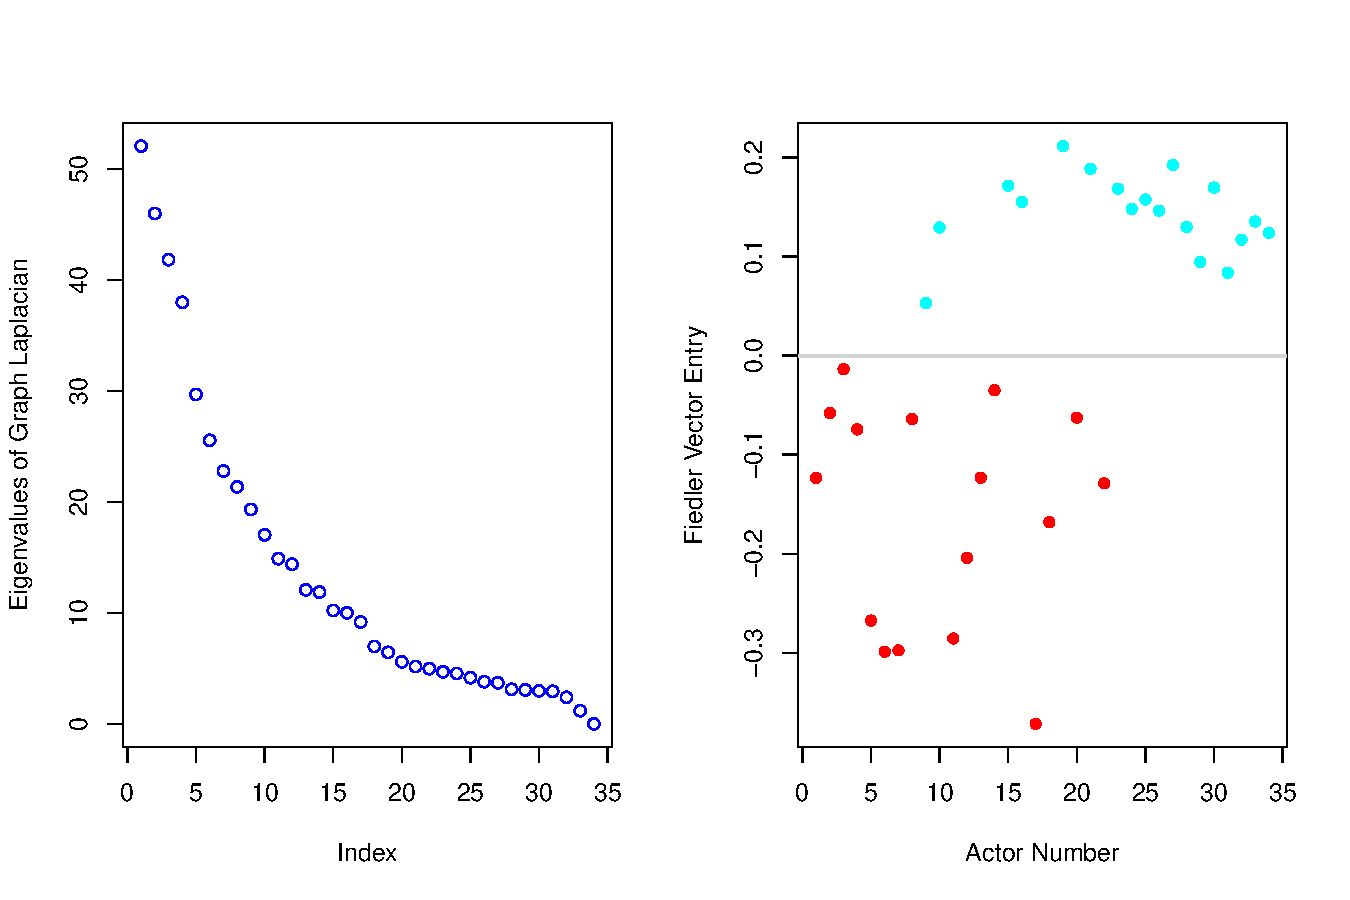
\includegraphics[width=.8\textwidth]{figures/laplacian_example-1} 

\end{knitrout}

\end{frame}

\begin{frame}[fragile]
  \frametitle{Clustering based on the first non null eigenvalue}
  
\begin{knitrout}\scriptsize
\definecolor{shadecolor}{rgb}{0.969, 0.969, 0.969}\color{fgcolor}\begin{kframe}
\begin{alltt}
\hlstd{hc} \hlkwb{<-} \hlkwd{cluster_leading_eigen}\hlstd{(karate)}
\hlkwd{plot}\hlstd{(hc,karate)}
\end{alltt}
\end{kframe}
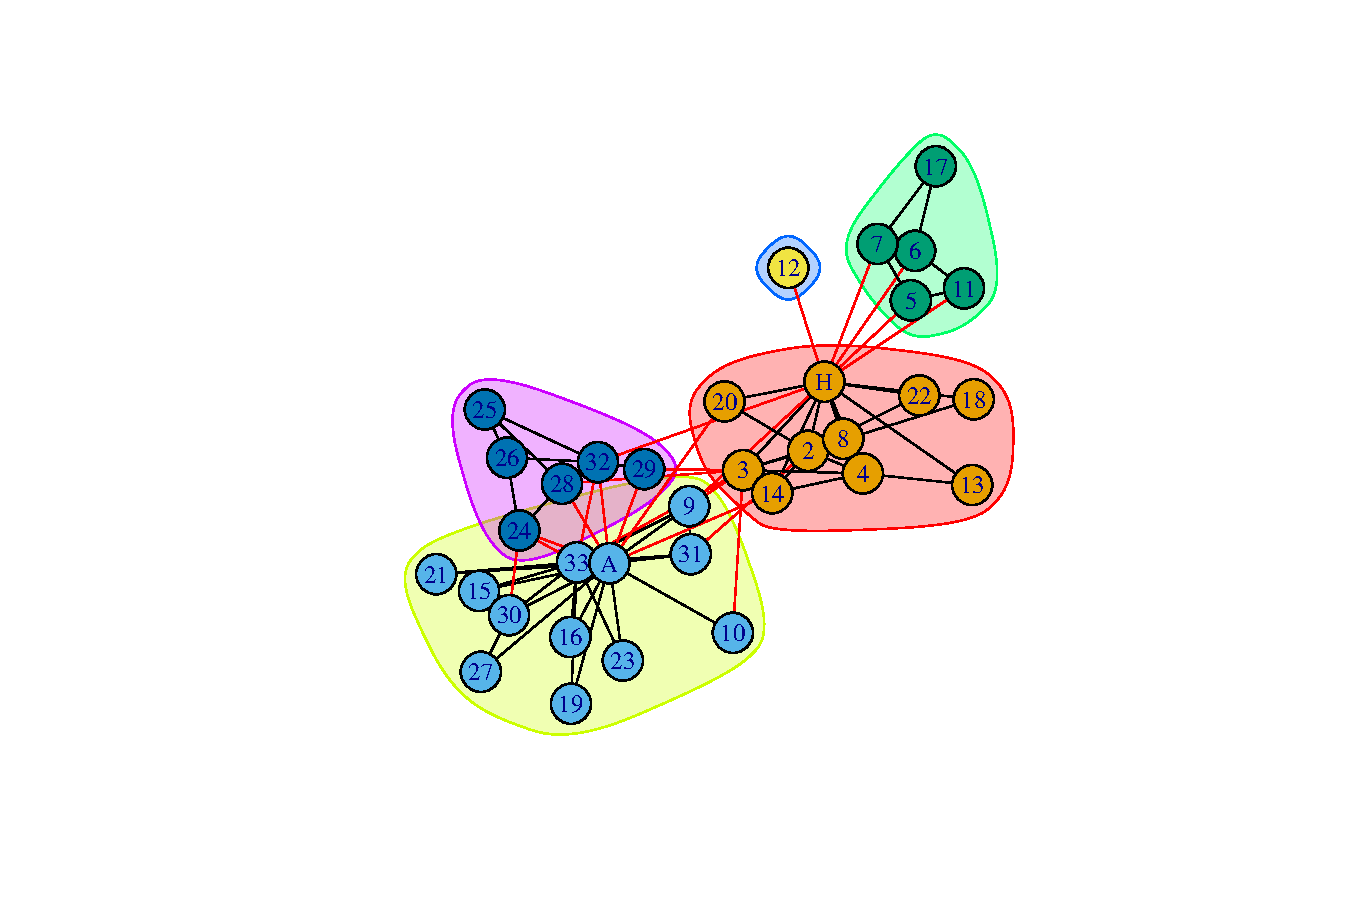
\includegraphics[width=.8\textwidth]{figures/unnamed-chunk-5-1} 

\end{knitrout}

\end{frame}


\end{document}
